\documentclass{article}

% Keep the official ICLR template isolated from the manuscript sources.
\makeatletter
\def\input@path{{template/}}
\makeatother

\usepackage{iclr2027_conference,times}
\input{template/math_commands.tex}

\usepackage{amsmath,amssymb,amsfonts,amsthm}
\usepackage{booktabs}
\usepackage{graphicx}
\usepackage{multirow}
\usepackage{algorithm}
\usepackage{algpseudocode}
\newtheorem{proposition}{Proposition}
\usepackage[hidelinks]{hyperref}
\usepackage{url}
% Shared table typography for the ICLR manuscript.
% Keep table-specific content in tables/ and presentation decisions here.

\newcommand{\meanstd}[2]{\mbox{#1\,{\scriptsize $\pm$\,#2}}}
\newcommand{\meanstdstacked}[2]{%
  \shortstack{#1\\[-1pt]{\tiny $\pm$\,#2}}%
}
\newcommand{\tablebest}[1]{\textbf{#1}}
\newcommand{\tablesecond}[1]{\underline{#1}}

% Default for compact ablations and diagnostic tables.
\newcommand{\tablebody}{%
  \centering
  \small
  \setlength{\tabcolsep}{5pt}%
  \renewcommand{\arraystretch}{1.08}%
}

% Use only when a table has many task columns.
\newcommand{\widetablebody}{%
  \centering
  \scriptsize
  \setlength{\tabcolsep}{2pt}%
  \renewcommand{\arraystretch}{1.04}%
}



% GATE-KD: Gauge-Aligned Target Embeddings for Knowledge Distillation
\title{Equivalent Representations Are Not Equivalent Distillation Targets}

% Authors must remain hidden while \iclrfinalcopy is commented out.
\author{Anonymous Authors}

% \iclrfinalcopy % Uncomment for camera-ready version, but NOT for submission.

\begin{document}

\maketitle

\begin{abstract}
Embedding distillation transfers knowledge from a large teacher to a smaller student, but their representations often differ in dimension and orientation. We propose GATE-KD, a final-embedding distillation method built around a comparable endpoint interface. A fixed principal-component projection selects a teacher subspace at the student dimension, while closed-form orthogonal Procrustes alignment follows the evolving student across epochs without altering the projected teacher geometry. We augment this interface with a native-space topological regularizer that matches degree-zero connectivity scales without requiring equal embedding dimensions. GATE-KD uses only cached final teacher embeddings and introduces no trainable alignment module. Under a label-free task-adapted protocol spanning three teacher--student configurations and nine sentence-level benchmarks, GATE-KD obtains the numerically highest aggregate score among the evaluated distilled students, exceeding the next-best baseline by 0.38--1.59 points while reducing measured GPU optimization-loop time by 62--74\%. Controlled analyses identify coordinate alignment as the primary mechanism, while the topological term provides a smaller complementary regularization effect. These results support a gauge-aligned endpoint interface as a competitive alternative to more complex pipelines in the task-adapted sentence-level regime studied here.
\end{abstract}

\section{Introduction}
\label{sec:introduction}

Text embedding models support retrieval, semantic similarity, clustering, and
classification, but the strongest encoders are often too costly for
latency- or memory-constrained deployment. Knowledge distillation offers a
natural route to compact embedding models by transferring supervision from a
frozen teacher to a smaller student
\citep{hinton2015distilling,reimers2020multilingual}. Unlike class logits,
however, embedding coordinates have no shared semantics across models. Teacher
and student representations may differ in dimension, orientation, and
architecture. Existing methods address this mismatch with learned projectors,
relational or contrastive objectives, and intermediate-layer supervision
\citep{park2019rkd,tian2020crd,xu2023distillcse,zhang2024jasper,truong2025emo,talas}.
Hierarchy-based transfer can be effective, but it requires access to internal
teacher representations and assumptions about cross-model layer
correspondence \citep{ko2023revisiting,kim2025layerselection}. This machinery
can obscure a more basic question: whether teacher and student endpoints have
first been expressed in comparable coordinates. We therefore study the endpoint
interface as a potential bottleneck in cross-dimensional distillation.

We test this hypothesis by centering the transfer mechanism on an
\emph{extrinsic interface} that expresses teacher representations in coordinates
the student can match pointwise. We augment this primary mechanism with an
\emph{intrinsic regularizer} defined on properties of the representation cloud
that do not depend on its coordinates or ambient dimension. This decomposition
leads to \textbf{GATE-KD}, Gauge Alignment and Topology for Embedding
Distillation. GATE-KD fits a fixed principal-component subspace to cached teacher
endpoints to provide a non-trainable reduction at the student width. Within the
retained subspace, orthogonal Procrustes alignment fits the orientation of the
teacher targets to the student's initial coordinates in closed form, without
changing sample correspondence or pairwise geometry.
Because projection cannot preserve all teacher geometry, GATE-KD adds a
degree-zero persistent-homology ($H_0$) summary regularizer that matches
distributions of connectivity scales in the native teacher and student spaces.
This coarse auxiliary summary is invariant to coordinates and ambient dimension;
it does not preserve sample-level neighborhoods or the full metric geometry. The resulting objective
supervises only the final student embedding, trains no alignment module, and
requires no online teacher forward pass during ordinary training.

Experiments across three teacher--student configurations and nine sentence-level
benchmarks under a label-free task-adapted protocol provide evidence consistent
with this endpoint-centered view. A per-minibatch rotation-invariant control
trails GATE-KD by 2.05 points; separate schedule controls suggest that
consistent corpus-level targets matter beyond allowing an adaptive rotation,
while periodic refitting provides only a smaller additional gain. Native-space
$H_0$ adds 0.53 points over endpoint-only training and performs best among the
evaluated structural controls and weights. Overall, GATE-KD obtains the
numerically highest aggregate score among the evaluated distilled students in
all three configurations, exceeding the next-best baseline by 0.38, 0.48, and
1.59 points. Within the measured minibatch optimization loop, it also records
the lowest update time and cumulative optimization time among the evaluated
methods in all three configurations. These results show that
final-embedding-only distillation can be competitive with the evaluated
hierarchy-based alternatives in the task-adapted sentence-level settings
studied here.

We make three contributions.
\begin{itemize}
    \item We formulate cross-dimensional embedding distillation around a
    comparable final-embedding interface, separating pointwise coordinate
    comparability from auxiliary coordinate-invariant structure.
    \item We introduce a fixed-reduction, closed-form gauge interface using only
    cached teacher endpoints, together with native-space $H_0$ regularization as
    a complementary signal and epoch-wise gauge refresh as a secondary
    optimization refinement.
    \item We provide a matched evaluation and controlled analyses that isolate
    gauge fitting, subspace construction, refitting, and $H_0$ connectivity-scale
    matching, clarifying
    which components account for the observed gains and the regime in which the
    conclusions apply.
\end{itemize}

\section{Related Work}
\label{sec:related-work}

Early text-embedding distillation directly regressed student sentence vectors
onto teacher outputs, showing that unlabeled text can provide dense supervision
without task annotations \citep{reimers2020multilingual}. Later methods enrich
this signal through contrastive objectives, specialized training recipes, and
teacher-compatible output spaces
\citep{gao2021distilcse,xu2023distillcse,simtde2023,zhang2024jasper,li2025ese,leaf}.
DistilCSE transfers a contrastive teacher through unlabeled-data distillation,
whereas SimTDE combines token- and sentence-level objectives with a projection
layer that relaxes equal-width requirements. LEALLA studies lightweight,
low-dimensional sentence encoders in a multilingual regime
\citep{lealla2023}. Data-centric systems
such as Gecko and jina-embeddings-v5-text additionally use generated, relabeled,
or task-targeted training data \citep{lee2024gecko,akram2026jina}; GATE-KD
instead holds the unlabeled corpus and downstream protocol fixed to isolate the
teacher--student interface. EmbedDistill combines endpoint matching with
relative geometric supervision for retrieval \citep{kim2023embeddistill}.
Other approaches exploit the representation hierarchy: EMO aligns token-level
relations and hidden states across tokenizers, while TALAS anchors upper student
layers to the teacher endpoint and self-distills lower layers
\citep{truong2025emo,talas}. MoL replaces rigid layer pairing with mixtures of
teacher layers, and feature-alignment distillation transfers intermediate states
and attention \citep{vu2026mol,wang2024feature}. Prior analyses also identify
overfitting in intermediate-layer distillation and limited sensitivity to layer
selection \citep{ko2023revisiting,kim2025layerselection}. GATE-KD studies the
complementary terminal-only regime using cached final teacher embeddings.

Dimension mismatch is commonly handled by mapping one representation space into
the other. HPD learns projection layers for compact sentence representations,
while broader studies show that projector parameterization and normalization
can materially affect student optimization
\citep{hpd,miles2024projector,chen2023projector}. Orthogonally constrained maps
preserve intra-batch similarity, whereas TCS uses PCA coordinates extracted from
cached teacher features \citep{vkd2024,tcs}. Representation-similarity work more
generally treats orthogonal transformations as natural equivalences because
they preserve inner products and distances, with Procrustes providing the
corresponding alignment
\citep{kornblith2019cka,williams2021shape,maystre2025procrustes}. Recent work
also formalizes supervision over representation equivalence classes
\citep{han2026equivalence}. Most closely related to our geometric motivation,
\citet{bhattarai2025shortcut} show that unconstrained projected matching can
achieve zero feature loss without preserving teacher Gram geometry, whereas
Procrustes alignment avoids this shortcut under their assumptions. GATE-KD uses
Procrustes as an epoch-wise coordinate-gauge update on a fixed PCA subspace
rather than as a trainable projector.

Coordinate-free objectives provide a complementary route to representation
structure. Relational, similarity-preserving, and contrastive distillation match
pairwise distances, Gram structure, or positive--negative relations
\citep{park2019rkd,tung2019similarity,tian2020crd}. Persistent homology extends
this view to multiscale properties of a point cloud. G-CRD studies local and
global graph-representation topology, while JDCEmb and DICE combine distillation
with geometry-shaping objectives in dialogue and diffusion settings
\citep{joshi2024representation,burykina2025jdcemb,zhou2026dice}. More directly,
TopKD transfers feature topology through approximate persistence images, and
topological-guidance distillation uses persistence features from multiple
teachers \citep{topkd2024,jeon2024topological}. Topologically regularized data
embeddings provide a broader framework for imposing prior topology on learned
low-dimensional representations \citep{heiter2023topological}. GATE-KD does not use topology as
a surrogate for full representation geometry or sample-wise supervision. Its
native-space regularizer matches sorted degree-zero persistence death times,
requiring neither shared coordinates nor equal ambient dimension, while the
explicit endpoint interface supplies the primary correspondence signal.

\section{Method}
\label{sec:method}

Let $f_T:\mathcal{X}\rightarrow\mathbb{R}^{d_T}$ be a frozen teacher and
$f_S(\cdot;\theta):\mathcal{X}\rightarrow\mathbb{R}^{d_S}$ a student with
parameters $\theta$ and $d_T>d_S$. We represent embeddings as row vectors
throughout. We run the teacher once over an unlabeled corpus
$\{x_i\}_{i=1}^{N}$ and cache its normalized final sentence embeddings
\begin{equation}
    \mathbf{t}_i=\operatorname{norm}\!\left(f_T(x_i)\right)
    \in\mathbb{S}^{d_T-1},
\end{equation}
where $\operatorname{norm}(\mathbf{x})=\mathbf{x}/\lVert\mathbf{x}\rVert_2$.
The corresponding student embedding is
$\mathbf{z}_i(\theta)=\operatorname{norm}(f_S(x_i;\theta))\in
\mathbb{S}^{d_S-1}$; we suppress $\theta$ when it is clear from context.
GATE-KD primarily transfers teacher knowledge through an
extrinsic interface that expresses each teacher endpoint in coordinates the
student can match pointwise. It augments this interface with an intrinsic
regularizer that requires neither shared coordinates nor equal ambient
dimension.

\subsection{Extrinsic Endpoint Interface}
\label{sec:method-targets}

\paragraph{Subspace selection.}
Let $\mu=N^{-1}\sum_i\mathbf{t}_i$. We fit the leading $d_S$ principal
directions of the centered cache and collect them as
$P_{\mathrm{PCA}}\in\mathbb{R}^{d_T\times d_S}$, with
$P_{\mathrm{PCA}}^\top P_{\mathrm{PCA}}=I_{d_S}$. Centering is used to
estimate the principal directions; in the evaluated recipe, the cached vectors
are not centered when the projection is applied. The normalized coordinates
before gauge alignment are
\begin{equation}
    \mathbf{y}_i
    =\operatorname{norm}\!\left(\mathbf{t}_iP_{\mathrm{PCA}}\right)
    \in\mathbb{S}^{d_S-1}.
    \label{eq:pca-target}
\end{equation}
The PCA subspace is fitted once on the full teacher cache and remains fixed
throughout training. Centering the cache to estimate covariance directions and
subtracting the mean when applying the interface are distinct operations: the
former selects a subspace, whereas the latter would make the target transform
affine and alter its angular geometry after row normalization. We use only the
former, preserving a linear endpoint interface. Appendix~\ref{app:pca-controls}
evaluates both choices together with whitening and random-subspace controls.

\paragraph{Gauge alignment.}
The basis used to express the retained subspace affects a pointwise loss even
though it does not affect the geometry within that subspace. We resolve this
coordinate ambiguity with orthogonal Procrustes alignment
\citep{schonemann1966procrustes,bhattarai2025shortcut}. We treat the orientation
as a nuisance coordinate variable rather than as teacher content. A gauge-fit
set $\mathcal{C}$ is selected before training and reused unchanged; in the main
experiments it is the complete distillation corpus. Let
$Y_{\mathcal{C}}$ contain $\mathbf{y}_i$ as rows and let
$Z_{\mathcal{C}}^{(e)}$ contain the corresponding student embeddings
$\mathbf{z}_i^{(e)}$ at the start of epoch $e$. We compute
\begin{equation}
    \begin{aligned}
    U\Sigma V^\top
      &=\operatorname{svd}\!\left(Y_{\mathcal{C}}^\top
        Z_{\mathcal{C}}^{(e)}\right),\\
    R^{(e)}=UV^\top
      &\in\underset{R\in O(d_S)}{\arg\min}\,
        \left\lVert Y_{\mathcal{C}}R-Z_{\mathcal{C}}^{(e)}\right\rVert_F^2.
    \end{aligned}
    \label{eq:gauge-alignment}
\end{equation}
The initialized student determines $R^{(0)}$. After each non-final epoch, we
re-encode the same gauge-fit sentences and refit the gauge for the following
epoch. The target used within epoch $e$ is therefore
\begin{equation}
    \boldsymbol{\tau}_i^{(e)}=\mathbf{y}_iR^{(e)}.
    \label{eq:target}
\end{equation}
Each target is fixed within an epoch. The refit is a closed-form coordinate
update rather than a learned projector. The minimizer in
Equation~\ref{eq:gauge-alignment} is unique exactly when the cross-covariance
$Y_{\mathcal{C}}^\top Z_{\mathcal{C}}^{(e)}$ has full rank
\citep{schonemann1966procrustes}; in directions with vanishing singular
values, $UV^\top$ is one of several minimizers and the returned orientation
depends on the SVD convention.

\paragraph{Relation to the endpoint objective.}
Because the rows of $Y_{\mathcal{C}}$ and $Z_{\mathcal{C}}^{(e)}$ have unit
norm, their cosine endpoint objective satisfies
\begin{equation}
    \frac{1}{|\mathcal{C}|}\sum_{i\in\mathcal{C}}
    \left(1-\left\langle\mathbf{z}_i^{(e)},\mathbf{y}_iR\right\rangle\right)
    =\frac{1}{2|\mathcal{C}|}
      \left\lVert Z_{\mathcal{C}}^{(e)}-Y_{\mathcal{C}}R\right\rVert_F^2.
    \label{eq:endpoint-procrustes}
\end{equation}
\begin{proposition}[Optimality and invariance of the fitted gauge]
\label{prop:gauge-optimality}
For row-normalized $Y_{\mathcal{C}}$ and $Z_{\mathcal{C}}^{(e)}$, the update
$R^{(e)}$ in Equation~\ref{eq:gauge-alignment} globally minimizes the gauge-fit
cosine endpoint loss over $O(d_S)$. Moreover, for every projected target matrix
$Y$ and every $R\in O(d_S)$,
\begin{equation}
    (Y R)(Y R)^\top=YY^\top.
    \label{eq:gauge-invariance}
\end{equation}
Thus fitting the gauge changes the coordinate presentation but not sample
correspondence, pairwise cosines, chord distances, or persistent-homology
signatures of the projected teacher targets.
\end{proposition}
The proof is given in Appendix~\ref{app:supporting-proofs}.

PCA supplies a fixed student-width subspace, while Procrustes determines how
that fixed geometry is presented in the student's coordinates. The update does
not select a new subspace or adapt the teacher's within-target geometry. At each
refit boundary, with the student fixed, it cannot increase the gauge-fit
endpoint loss and leaves the native-space $H_0$ term unchanged. This conditional
guarantee does not imply monotonic epoch-to-epoch training because the student
changes between refits.

\subsection{Native-Space \texorpdfstring{$H_0$}{H0} Persistence-Summary Regularization}
\label{sec:method-topology}

The endpoint interface can reproduce only the geometry retained after
projection. Although $P_{\mathrm{PCA}}$ has orthonormal columns,
$P_{\mathrm{PCA}}P_{\mathrm{PCA}}^\top$ is a rank-$d_S$ projector, so the
cosine Gram matrix of the normalized coordinates in
Equation~\ref{eq:pca-target} need not equal that of the original teacher
embeddings. This loss of geometry is unavoidable whenever the normalized
teacher cache has rank above the student width.
\begin{proposition}[Rank-relaxed lower bound on Gram distortion]
\label{prop:gram-lower-bound}
Let $T\in\mathbb{R}^{N\times d_T}$ collect the normalized teacher cache
embeddings, with singular values
$\sigma_1(T)\geq\cdots\geq\sigma_r(T)>0$. For every $Z\in
\mathbb{R}^{N\times d_S}$ collecting student embeddings of the same $N$
sentences,
\begin{equation}
    \left\lVert TT^\top-ZZ^\top\right\rVert_F^2
    \geq \sum_{j>d_S}\sigma_j(T)^4.
    \label{eq:gram-lower-bound}
\end{equation}
Thus exact preservation of the teacher cosine Gram matrix is impossible when
$\operatorname{rank}(T)>d_S$. The bound relaxes the unit-diagonal constraint on
$ZZ^\top$ and therefore need not be tight for normalized student embeddings.
\end{proposition}
The proof is given in Appendix~\ref{app:supporting-proofs}.

Rather than attempting to reconstruct the full teacher Gram geometry, which is
generally impossible at student rank, we match a lower-complexity,
coordinate-free summary of its connectivity scales. We therefore add a
persistence-summary regularizer defined directly in the teacher's native space.

For a minibatch $\mathcal{B}\subseteq\{1,\ldots,N\}$ of size
$|\mathcal{B}|=B$, we use the chord distance
\begin{equation}
    d(\mathbf{u},\mathbf{v})
    =\sqrt{2-2\langle\mathbf{u},\mathbf{v}\rangle}.
\end{equation}
We parameterize the Vietoris--Rips filtration by the distance threshold: an
edge enters at scale $a$ when its distance is at most $a$.
The $B-1$ finite death times of degree-zero Vietoris--Rips persistence are the
edge weights of the point cloud's minimum spanning tree
\citep{hofer2020topologically}. Let
$q^S_{(1)}\leq\cdots\leq q^S_{(B-1)}$ and
$q^T_{(1)}\leq\cdots\leq q^T_{(B-1)}$ denote the sorted death times
of the student embeddings $\{\mathbf{z}_i:i\in\mathcal{B}\}$ and the original
teacher embeddings $\{\mathbf{t}_i:i\in\mathcal{B}\}$. We define
\begin{equation}
    \mathcal{L}_{H_0}
    =\frac{1}{B-1}\sum_{j=1}^{B-1}
      \left(q^S_{(j)}-q^T_{(j)}\right)^2.
    \label{eq:topological-loss}
\end{equation}
For a precise interpretation, define the empirical distributions of finite
connectivity scales
\begin{equation}
    \nu_S=\frac{1}{B-1}\sum_{j=1}^{B-1}\delta_{q^S_{(j)}},
    \qquad
    \nu_T=\frac{1}{B-1}\sum_{j=1}^{B-1}\delta_{q^T_{(j)}},
\end{equation}
where $\delta_a$ denotes a Dirac mass at $a$.
\begin{proposition}[Transport interpretation and stability]
\label{prop:h0-transport-stability}
The $H_0$ loss equals the squared one-dimensional Wasserstein distance between
the empirical death-scale measures,
\begin{equation}
    \mathcal{L}_{H_0}=W_2^2(\nu_S,\nu_T).
    \label{eq:topological-wasserstein}
\end{equation}
Moreover, if the two distance matrices on the corresponding batch satisfy
\begin{equation}
    \epsilon=\max_{i,j\in\mathcal{B}}
    \left|d(\mathbf{z}_i,\mathbf{z}_j)
          -d(\mathbf{t}_i,\mathbf{t}_j)\right|,
\end{equation}
then $\mathcal{L}_{H_0}\leq\epsilon^2$.
\end{proposition}
The proof is given in Appendix~\ref{app:supporting-proofs}.

The teacher diagram is computed from $\mathbf{t}_i\in\mathbb{R}^{d_T}$ rather
than $\mathbf{y}_i$ or $\boldsymbol{\tau}_i^{(e)}$. The loss therefore needs
neither a projection nor a shared orientation. It is differentiable almost
everywhere away from distance ties and changes in the active minimum spanning
tree \citep{hofer2019connectivity}. In implementation, the discrete tree
selection and sorting permutation are treated as fixed during backpropagation,
while gradients flow through the selected student edge weights.
The stability result is one-way. Equation~\ref{eq:topological-loss} matches the
multiset of $H_0$ death times but does not impose correspondence between
individual minimum-spanning-tree edges, recover the full metric geometry, or
preserve higher-dimensional topological features.

Algorithm~\ref{alg:h0-loss} makes the nonsmooth implementation explicit. The
teacher branch is evaluated without gradients. On the student branch, the MST
edge selection and sorting permutation are detached, while the selected edge
weights remain differentiable. Exact distance ties are passed to SciPy in
row-major upper-triangular order. Although the selected active tree can depend
on this library tie-break, every valid MST has the same sorted multiset of edge
weights; the backward pass follows the particular active tree returned in that
forward pass.

\begin{algorithm}[t]
\caption{Native-space $H_0$ connectivity-scale loss for one minibatch}
\label{alg:h0-loss}
\begin{algorithmic}[1]
\Require Row-normalized teacher and student batches $T_{\mathcal B}$ and
$Z_{\mathcal B}$; numerical floor $\varepsilon$.
\For{$A\in\{T_{\mathcal B},Z_{\mathcal B}\}$}
    \State Compute $G\gets AA^\top$ in FP32 and symmetrize
    $G\gets(G+G^\top)/2$.
    \State Compute $D_{ij}\gets\sqrt{\max(2-2G_{ij},\varepsilon)}$ and set
    $D_{ii}\gets0$.
    \State On a detached CPU float64 copy, add the same positive constant to
    every off-diagonal edge and select an undirected MST with SciPy from the
    upper triangle.
    \State Gather the selected weights from the unshifted $D$ and sort them to
    obtain $q^A_{(1:B-1)}$.
\EndFor
\State \Return $(B-1)^{-1}\sum_{j=1}^{B-1}(q^Z_{(j)}-q^T_{(j)})^2$.
\end{algorithmic}
\end{algorithm}

\subsection{Objective and Alternating Optimization}
\label{sec:method-objective}

The endpoint loss for the same training minibatch $\mathcal{B}$ is
\begin{equation}
    \mathcal{L}_{\mathrm{end}}^{(e)}
    =\frac{1}{B}\sum_{i\in\mathcal{B}}
      \left(1-\left\langle
      \mathbf{z}_i,\boldsymbol{\tau}_i^{(e)}\right\rangle\right).
    \label{eq:endpoint-loss}
\end{equation}
GATE-KD optimizes the two-term objective
\begin{equation}
    \mathcal{L}^{(e)}
    =\mathcal{L}_{\mathrm{end}}^{(e)}
    +\lambda_{\mathrm{topo}}\mathcal{L}_{H_0}.
    \label{eq:objective}
\end{equation}
Here, $\mathcal{L}_{H_0}$ is evaluated on the same minibatch using the student
embeddings and the corresponding unprojected teacher embeddings.

Optimization alternates between stochastic updates of the student parameters
and exact updates of the nuisance coordinate gauge. It can be viewed as an
inexact block-coordinate procedure over $\theta$ and $R\in O(d_S)$: with the
student fixed, Equation~\ref{eq:gauge-alignment} solves the endpoint term
exactly over $R$ on $\mathcal{C}$; with the gauge fixed, stochastic minibatch
updates modify $\theta$. During epoch $e$, $R^{(e)}$ is held
fixed while the student is optimized with Equation~\ref{eq:objective}. After
epoch $e$, unless it is the final epoch, the updated student re-encodes
$\mathcal{C}$ and Equation~\ref{eq:gauge-alignment} produces $R^{(e+1)}$ for
the next epoch. The $H_0$ term is unaffected by these gauge updates because it
is computed from the native teacher embeddings.

Teacher embeddings and the PCA subspace are computed once before student
optimization. Ordinary training steps use the cached teacher embeddings and
require no online teacher forward pass. Each gauge update adds one student pass
over the gauge-fit set and an SVD of a $d_S\times d_S$ matrix. This joint view
does not by itself imply that repeated refitting improves generalization; the
controlled analysis in Section~\ref{sec:analysis-interface} treats it as a
secondary refinement beyond the initially fitted gauge.

\section{Experiments}
\label{sec:experiments}

\subsection{Experimental Setup}
\label{sec:exp-setup}

\paragraph{Teacher--student configurations.}
We adopt the three teacher--student pairs evaluated by TALAS \citep{talas}.
They comprise Qwen3-Embedding-4B $\rightarrow$ BERT-base, BGE-M3
$\rightarrow$ MiniLMv2-L6-H768, and Qwen3-Embedding-0.6B $\rightarrow$
MiniLMv2-L6-H384
\citep{devlin2019bert,wang2021minilmv2,chen2024m3,zhang2025qwen3embedding}.
These settings span students from 22M to 109M parameters and embedding
bottlenecks of $2560\rightarrow768$, $1024\rightarrow768$, and
$1024\rightarrow384$, respectively. The Qwen teachers use last-token pooling,
whereas BGE-M3 uses CLS pooling.

\paragraph{Distillation corpus.}
Following TALAS \citep{talas}, every method uses the same corpus of about 5K
unlabeled training texts from each of Emotion, WiC, and STS-B; no labels are
used. We call these three benchmarks source tasks and the other six non-source
tasks. ``Non-source'' denotes only absence from this corpus, not unrestricted
domain shift.

\paragraph{Baselines.}
The baselines span relational transfer (RKD), multi-stage endpoint distillation
(Stella), cross-tokenizer or dual-space transfer (CDM, DSKD), and hidden-state
alignment (EMO, TALAS)
\citep{park2019rkd,zhang2024jasper,chen2025cdm,zhang2024dskd,truong2025emo,talas}.
All share the corpus, model pairs, evaluator, five-epoch budget, batch size 128,
and learning-rate grid while retaining method-specific components. This is a
controlled-budget comparison, not an upper bound after per-pair tuning; full
implementation choices appear in Appendix~\ref{app:training-hyperparameters}.

\paragraph{Evaluation protocol.}
We evaluate frozen embeddings on classification (Banking77, Emotion, Tweet;
macro-F1), pair classification (MRPC, SciTail, WiC; average precision from
cosine similarity), and semantic similarity (SICK, STS12, STS-B; Spearman
correlation). Metrics are multiplied by 100 and averaged over three seeds.
Avg. is the unweighted mean of nine heterogeneous task metrics and is therefore
a descriptive index; Src and Non-src separately average the three source and
six non-source tasks.

\subsection{Main Results}
\label{sec:main-results}

\begin{table}[t]
    \caption{Nine-task results on the 15K distillation corpus. Distilled
    students report mean $\pm$ sample standard deviation over three seeds;
    best and second-best results are bold and underlined. GATE-KD uses
    $\lambda_{H_0}=0.5$.}
    \label{tab:main-results}
    \widetablebody
    \begin{tabular}{@{}lcccccccccccc@{}}
        \toprule
        & \multicolumn{3}{c}{Classification (F1)}
        & \multicolumn{3}{c}{Pair Classification (AP)}
        & \multicolumn{3}{c}{STS (Spearman)}
        & \multicolumn{3}{c}{Averages} \\
        \cmidrule(lr){2-4}\cmidrule(lr){5-7}\cmidrule(lr){8-10}\cmidrule(lr){11-13}
        Method & Banking77 & Tweet & Emotion & MRPC & SciTail & WiC
        & SICK & STS12 & STS-B & Src & Non-src & All \\
        \midrule
        \multicolumn{13}{@{}c}{\textit{(a) Qwen3-Embedding-4B $\rightarrow$ BERT-base (109M)}} \\
        \midrule
        Teacher
        & 93.26 & 71.04 & 69.08 & 84.80 & 91.77 & 66.79
        & 83.43 & 82.55 & 86.87 & 74.25 & 84.48 & 81.07 \\
        Student (pre-KD)
        & 84.33 & 67.08 & 47.79 & 77.36 & 67.74 & 59.22
        & 42.43 & 21.54 & 20.29 & 42.43 & 60.08 & 54.20 \\
        \midrule
        RKD
        & \meanstdstacked{89.76}{0.11} & \meanstdstacked{70.90}{0.31} & \meanstdstacked{59.98}{0.05}
        & \meanstdstacked{81.94}{0.26} & \meanstdstacked{75.59}{0.13} & \meanstdstacked{69.02}{0.18}
        & \meanstdstacked{72.93}{0.07} & \meanstdstacked{67.84}{0.18} & \meanstdstacked{73.72}{0.08}
        & \meanstdstacked{67.57}{0.05} & \meanstdstacked{76.49}{0.07} & \meanstdstacked{73.52}{0.06} \\
        Stella
        & \meanstdstacked{88.48}{0.30} & \meanstdstacked{68.94}{0.17} & \meanstdstacked{53.69}{0.50}
        & \meanstdstacked{83.95}{0.10} & \meanstdstacked{75.39}{0.54} & \meanstdstacked{\tablebest{71.93}}{0.09}
        & \meanstdstacked{69.87}{0.64} & \meanstdstacked{64.39}{0.21} & \meanstdstacked{70.86}{0.36}
        & \meanstdstacked{65.49}{0.17} & \meanstdstacked{75.17}{0.13} & \meanstdstacked{71.95}{0.06} \\
        CDM
        & \meanstdstacked{88.13}{0.23} & \meanstdstacked{69.03}{0.20} & \meanstdstacked{52.83}{0.50}
        & \meanstdstacked{83.00}{0.06} & \meanstdstacked{77.10}{0.27} & \meanstdstacked{71.84}{0.09}
        & \meanstdstacked{67.89}{0.37} & \meanstdstacked{61.06}{0.37} & \meanstdstacked{69.19}{0.42}
        & \meanstdstacked{64.62}{0.28} & \meanstdstacked{74.37}{0.12} & \meanstdstacked{71.12}{0.18} \\
        DSKD
        & \meanstdstacked{87.97}{0.16} & \meanstdstacked{68.90}{0.28} & \meanstdstacked{53.07}{0.31}
        & \meanstdstacked{83.03}{0.15} & \meanstdstacked{76.98}{0.59} & \meanstdstacked{\tablesecond{71.86}}{0.08}
        & \meanstdstacked{67.77}{0.66} & \meanstdstacked{61.11}{0.26} & \meanstdstacked{69.55}{0.12}
        & \meanstdstacked{64.83}{0.12} & \meanstdstacked{74.29}{0.14} & \meanstdstacked{71.14}{0.10} \\
        EMO
        & \meanstdstacked{86.89}{0.07} & \meanstdstacked{68.99}{0.11} & \meanstdstacked{52.02}{1.09}
        & \meanstdstacked{79.74}{0.12} & \meanstdstacked{76.37}{0.35} & \meanstdstacked{69.62}{0.16}
        & \meanstdstacked{67.89}{0.09} & \meanstdstacked{56.46}{0.47} & \meanstdstacked{64.54}{0.50}
        & \meanstdstacked{62.06}{0.49} & \meanstdstacked{72.72}{0.15} & \meanstdstacked{69.17}{0.24} \\
        TALAS
        & \meanstdstacked{\tablesecond{90.53}}{0.09} & \meanstdstacked{\tablesecond{73.77}}{0.21} & \meanstdstacked{\tablesecond{68.47}}{0.34}
        & \meanstdstacked{\tablebest{85.38}}{0.05} & \meanstdstacked{\tablebest{81.83}}{0.21} & \meanstdstacked{69.59}{0.14}
        & \meanstdstacked{\tablesecond{76.79}}{0.06} & \meanstdstacked{\tablesecond{70.79}}{0.19} & \meanstdstacked{\tablebest{78.50}}{0.08}
        & \meanstdstacked{\tablebest{72.19}}{0.07} & \meanstdstacked{\tablesecond{79.85}}{0.07} & \meanstdstacked{\tablesecond{77.29}}{0.04} \\
        \midrule
        \tablebest{GATE-KD}
        & \meanstdstacked{\tablebest{90.60}}{0.21} & \meanstdstacked{\tablebest{73.86}}{0.10} & \meanstdstacked{\tablebest{69.48}}{0.22}
        & \meanstdstacked{\tablesecond{85.31}}{0.11} & \meanstdstacked{\tablesecond{80.23}}{0.13} & \meanstdstacked{68.19}{0.12}
        & \meanstdstacked{\tablebest{77.80}}{0.14} & \meanstdstacked{\tablebest{75.15}}{0.07} & \meanstdstacked{\tablesecond{78.44}}{0.16}
        & \meanstdstacked{\tablesecond{72.04}}{0.08} & \meanstdstacked{\tablebest{80.49}}{0.03} & \meanstdstacked{\tablebest{77.67}}{0.03} \\
        \midrule
        \multicolumn{13}{@{}c}{\textit{(b) BGE-M3 $\rightarrow$ MiniLMv2-H768 (66M)}} \\
        \midrule
        Teacher
        & 93.49 & 73.75 & 69.03 & 85.80 & 91.87 & 61.46
        & 79.18 & 78.74 & 84.86 & 71.78 & 83.81 & 79.80 \\
        Student (pre-KD)
        & 81.18 & 71.30 & 48.85 & 79.66 & 65.06 & 60.89
        & 49.46 & 26.76 & 24.12 & 44.62 & 62.24 & 56.36 \\
        \midrule
        RKD
        & \meanstdstacked{89.14}{0.09} & \meanstdstacked{73.29}{0.09} & \meanstdstacked{\tablesecond{62.23}}{0.27}
        & \meanstdstacked{84.35}{0.06} & \meanstdstacked{78.74}{0.11} & \meanstdstacked{65.02}{0.10}
        & \meanstdstacked{73.20}{0.19} & \meanstdstacked{65.02}{0.29} & \meanstdstacked{71.97}{0.38}
        & \meanstdstacked{66.41}{0.07} & \meanstdstacked{77.29}{0.06} & \meanstdstacked{73.66}{0.04} \\
        Stella
        & \meanstdstacked{86.82}{0.28} & \meanstdstacked{70.06}{0.12} & \meanstdstacked{56.61}{0.74}
        & \meanstdstacked{83.02}{0.12} & \meanstdstacked{74.63}{0.12} & \meanstdstacked{\tablebest{69.72}}{0.05}
        & \meanstdstacked{69.08}{0.20} & \meanstdstacked{63.14}{0.28} & \meanstdstacked{67.10}{0.10}
        & \meanstdstacked{64.47}{0.27} & \meanstdstacked{74.46}{0.05} & \meanstdstacked{71.13}{0.11} \\
        CDM
        & \meanstdstacked{87.82}{0.19} & \meanstdstacked{69.99}{0.09} & \meanstdstacked{58.32}{0.51}
        & \meanstdstacked{83.44}{0.07} & \meanstdstacked{75.56}{0.40} & \meanstdstacked{\tablesecond{69.70}}{0.02}
        & \meanstdstacked{65.93}{0.16} & \meanstdstacked{60.84}{0.34} & \meanstdstacked{65.31}{0.15}
        & \meanstdstacked{64.45}{0.13} & \meanstdstacked{73.93}{0.06} & \meanstdstacked{70.77}{0.02} \\
        DSKD
        & \meanstdstacked{87.70}{0.16} & \meanstdstacked{70.35}{0.32} & \meanstdstacked{59.71}{0.61}
        & \meanstdstacked{82.99}{0.18} & \meanstdstacked{75.58}{0.12} & \meanstdstacked{69.59}{0.04}
        & \meanstdstacked{65.36}{0.37} & \meanstdstacked{61.21}{0.31} & \meanstdstacked{65.02}{0.18}
        & \meanstdstacked{64.77}{0.27} & \meanstdstacked{73.87}{0.10} & \meanstdstacked{70.83}{0.11} \\
        EMO
        & \meanstdstacked{87.54}{0.18} & \meanstdstacked{71.03}{0.14} & \meanstdstacked{58.52}{0.30}
        & \meanstdstacked{82.46}{0.18} & \meanstdstacked{74.73}{0.58} & \meanstdstacked{69.20}{0.22}
        & \meanstdstacked{64.71}{0.55} & \meanstdstacked{56.89}{0.27} & \meanstdstacked{61.25}{0.03}
        & \meanstdstacked{62.99}{0.19} & \meanstdstacked{72.89}{0.10} & \meanstdstacked{69.59}{0.12} \\
        TALAS
        & \meanstdstacked{\tablesecond{89.83}}{0.09} & \meanstdstacked{\tablebest{74.70}}{0.09} & \meanstdstacked{61.65}{0.23}
        & \meanstdstacked{\tablebest{86.62}}{0.05} & \meanstdstacked{\tablesecond{80.85}}{0.22} & \meanstdstacked{66.72}{0.07}
        & \meanstdstacked{\tablesecond{75.40}}{0.10} & \meanstdstacked{\tablesecond{67.08}}{0.31} & \meanstdstacked{\tablesecond{77.08}}{0.01}
        & \meanstdstacked{\tablesecond{68.48}}{0.07} & \meanstdstacked{\tablesecond{79.08}}{0.08} & \meanstdstacked{\tablesecond{75.55}}{0.06} \\
        \midrule
        \tablebest{GATE-KD}
        & \meanstdstacked{\tablebest{90.17}}{0.05} & \meanstdstacked{\tablesecond{73.74}}{0.24} & \meanstdstacked{\tablebest{64.83}}{0.72}
        & \meanstdstacked{\tablesecond{86.42}}{0.09} & \meanstdstacked{\tablebest{80.97}}{0.08} & \meanstdstacked{65.47}{0.09}
        & \meanstdstacked{\tablebest{76.77}}{0.03} & \meanstdstacked{\tablebest{68.27}}{0.04} & \meanstdstacked{\tablebest{77.63}}{0.12}
        & \meanstdstacked{\tablebest{69.31}}{0.21} & \meanstdstacked{\tablebest{79.39}}{0.06} & \meanstdstacked{\tablebest{76.03}}{0.11} \\
        \midrule
        \multicolumn{13}{@{}c}{\textit{(c) Qwen3-Embedding-0.6B $\rightarrow$ MiniLMv2-H384 (22M)}} \\
        \midrule
        Teacher
        & 92.51 & 71.28 & 65.80 & 83.38 & 90.09 & 66.84
        & 80.65 & 77.11 & 84.59 & 72.41 & 82.50 & 79.14 \\
        Student (pre-KD)
        & 67.03 & 69.45 & 42.90 & 78.39 & 64.55 & 59.58
        & 47.60 & 21.96 & 22.08 & 41.52 & 58.16 & 52.62 \\
        \midrule
        RKD
        & \meanstdstacked{\tablesecond{86.76}}{0.07} & \meanstdstacked{69.87}{0.21} & \meanstdstacked{56.31}{0.35}
        & \meanstdstacked{81.70}{0.03} & \meanstdstacked{76.03}{0.20} & \meanstdstacked{\tablesecond{68.56}}{0.22}
        & \meanstdstacked{69.21}{0.18} & \meanstdstacked{64.26}{0.19} & \meanstdstacked{70.25}{0.21}
        & \meanstdstacked{65.04}{0.20} & \meanstdstacked{74.64}{0.09} & \meanstdstacked{71.44}{0.10} \\
        Stella
        & \meanstdstacked{84.04}{0.04} & \meanstdstacked{68.73}{0.44} & \meanstdstacked{52.41}{0.28}
        & \meanstdstacked{81.50}{0.12} & \meanstdstacked{72.26}{0.32} & \meanstdstacked{\tablebest{68.65}}{0.16}
        & \meanstdstacked{64.64}{0.19} & \meanstdstacked{60.59}{0.12} & \meanstdstacked{64.27}{0.20}
        & \meanstdstacked{61.78}{0.13} & \meanstdstacked{71.96}{0.13} & \meanstdstacked{68.57}{0.10} \\
        CDM
        & \meanstdstacked{84.74}{0.21} & \meanstdstacked{69.52}{0.20} & \meanstdstacked{53.76}{0.95}
        & \meanstdstacked{81.15}{0.14} & \meanstdstacked{72.86}{0.30} & \meanstdstacked{68.29}{0.11}
        & \meanstdstacked{63.98}{0.36} & \meanstdstacked{60.43}{0.22} & \meanstdstacked{63.52}{0.24}
        & \meanstdstacked{61.86}{0.43} & \meanstdstacked{72.11}{0.19} & \meanstdstacked{68.69}{0.27} \\
        DSKD
        & \meanstdstacked{84.76}{0.10} & \meanstdstacked{69.56}{0.20} & \meanstdstacked{53.14}{0.29}
        & \meanstdstacked{81.15}{0.01} & \meanstdstacked{72.81}{0.09} & \meanstdstacked{68.33}{0.04}
        & \meanstdstacked{63.78}{0.06} & \meanstdstacked{60.24}{0.19} & \meanstdstacked{63.53}{0.18}
        & \meanstdstacked{61.67}{0.03} & \meanstdstacked{72.05}{0.06} & \meanstdstacked{68.59}{0.04} \\
        EMO
        & \meanstdstacked{83.54}{0.31} & \meanstdstacked{69.31}{0.06} & \meanstdstacked{54.48}{0.27}
        & \meanstdstacked{80.87}{0.13} & \meanstdstacked{72.00}{0.16} & \meanstdstacked{67.89}{0.09}
        & \meanstdstacked{62.19}{0.16} & \meanstdstacked{57.04}{0.17} & \meanstdstacked{61.24}{0.23}
        & \meanstdstacked{61.20}{0.09} & \meanstdstacked{70.82}{0.07} & \meanstdstacked{67.62}{0.02} \\
        TALAS
        & \meanstdstacked{86.39}{0.13} & \meanstdstacked{\tablesecond{71.81}}{0.11} & \meanstdstacked{\tablesecond{58.40}}{0.30}
        & \meanstdstacked{\tablebest{84.25}}{0.03} & \meanstdstacked{\tablesecond{79.29}}{0.11} & \meanstdstacked{66.82}{0.02}
        & \meanstdstacked{\tablesecond{70.42}}{0.10} & \meanstdstacked{\tablesecond{68.08}}{0.22} & \meanstdstacked{\tablesecond{73.34}}{0.10}
        & \meanstdstacked{\tablesecond{66.19}}{0.11} & \meanstdstacked{\tablesecond{76.71}}{0.04} & \meanstdstacked{\tablesecond{73.20}}{0.06} \\
        \midrule
        \tablebest{GATE-KD}
        & \meanstdstacked{\tablebest{87.77}}{0.07} & \meanstdstacked{\tablebest{72.30}}{0.19} & \meanstdstacked{\tablebest{63.45}}{0.43}
        & \meanstdstacked{\tablesecond{84.19}}{0.03} & \meanstdstacked{\tablebest{81.56}}{0.16} & \meanstdstacked{68.17}{0.05}
        & \meanstdstacked{\tablebest{72.59}}{0.03} & \meanstdstacked{\tablebest{68.91}}{0.03} & \meanstdstacked{\tablebest{74.79}}{0.05}
        & \meanstdstacked{\tablebest{68.80}}{0.16} & \meanstdstacked{\tablebest{77.89}}{0.01} & \meanstdstacked{\tablebest{74.86}}{0.06} \\
        \bottomrule
    \end{tabular}
\end{table}


GATE-KD has the highest numerical Avg. in all three configurations, exceeding
the next-best baseline by 0.38, 0.48, and 1.59 points. The first two are small
three-seed differences; the compact result is both larger and broader. Relative
to TALAS, GATE-KD is higher on 5/9, 6/9, and 8/9 task means, respectively
(Appendix~\ref{app:task-mean-differences}), and ranks first in 18 of 27
task--configuration comparisons overall. Pair classification remains mixed.

In configuration (c), endpoint-only GATE-KD reaches $74.26\pm0.02$, already
1.06 points above TALAS; $H_0$ adds 0.53 points. Thus the endpoint interface,
not the auxiliary, supplies most of the compact gain. The result also shows
that intermediate teacher states were not required in this comparison, without
implying that intermediate supervision is generally inferior.

On five corpus-disjoint BEIR retrieval benchmarks, GATE-KD ranks first on
average in (b) and (c) and second in (a), although all students remain below
their teachers (Appendix~\ref{app:retrieval-15k}). This is a transfer guardrail,
not a substitute for benchmark-disjoint general-text distillation.

\FloatBarrier

\section{What Drives GATE-KD?}
\label{sec:analysis}

We organize the analysis around two empirical observations. First, within the
evaluated controls, the endpoint interface obtains most of its numerical gain
after establishing fitted coordinate comparability;
the particular fixed subspace and repeated gauge updates are secondary design
choices. Second, native-space $H_0$ provides a smaller complementary signal
rather than replacing sample-wise endpoint supervision. Unless stated
otherwise, controls use configuration (c), whose 384-dimensional student has
the strongest width bottleneck. The variants come from matched rerun suites;
their GATE-KD reference rows repeat configuration (c) from the main sweep for
consistency. Extended controls are grouped by claim in
Appendices~\ref{app:endpoint-analysis} and~\ref{app:structural-analysis}.

\subsection{Fitted Coordinate Comparability Explains Most of the Endpoint Gain}
\label{sec:analysis-interface}

Table~\ref{tab:gauge-mechanism} holds the PCA subspace and full GATE-KD
objective (endpoint supervision plus native-space $H_0$) fixed while varying
how the endpoint coordinates are treated. The unaligned row trains directly
against the fixed PCA coordinates and therefore doubles as the matched
PCA-only endpoint baseline, the sentence-embedding analogue of the TCS target
construction \citep{tcs}. In configuration (c), no alignment,
a random orientation, a fixed fitted gauge, one refit, and epoch-wise
Procrustes reach 72.51, 73.02, 74.63, 74.64, and 74.79 Avg., respectively. The
additional invariant control directly minimizes the endpoint loss over an
orthogonal rotation on every minibatch and reaches $72.74\pm0.07$. It improves
only marginally over the unaligned controls and trails epoch-wise Procrustes by
2.05 points. Separately, within the gauge-schedule controls, the fixed fitted
gauge gains 2.12 points over no alignment and retains all but 0.16 points of the
epoch-wise result. Taken together, these results argue against explaining the
gain by merely weakening pointwise matching through a student-adaptive
rotation. They are instead consistent with the benefit coming from one fitted
orientation, shared across minibatches, that is consistent with the student's
initial coordinates. We note what these controls do not isolate: because
$R^{(0)}$ is fitted to the initialized student, the schedule controls cannot
separate a resolved cross-model coordinate mismatch from a target orientation
that merely makes early optimization easier for that particular
initialization. A control that fits $R^{(0)}$ on one initialization and trains
independently initialized students against that fixed orientation would
separate the two readings; we leave it to future work and interpret the gauge
here as an empirically useful optimization device rather than as a
transferable coordinate system.

% Control rows: review_h0_pca_controls_20260906-143901, gauge family.
% Epoch-wise Procrustes reference: main-results configuration (c).
% Invariant row: invariant_procrustes_c_3seeds_20260906-215912.
\begin{table}[!t]
    \centering
    \caption{Compact orientation treatments under the full objective (mean
    $\pm$ sample standard deviation, three seeds).}
    \label{tab:gauge-mechanism}
    \small
    \newcommand{\gcell}[2]{#1{\tiny $\pm$ #2}}
    \setlength{\tabcolsep}{5pt}
    \begin{tabular}{@{}lcc@{}}
        \toprule
        Orientation treatment & Updates & Config. (c) Avg. $\uparrow$ \\
        \midrule
        None (fixed PCA target) & 0 & \gcell{72.51}{0.05} \\
        Random orthogonal & 0 & \gcell{73.02}{0.05} \\
        Per-minibatch invariant & Every step & \gcell{72.74}{0.07} \\
        Fixed $R^{(0)}$ & 0 & \gcell{74.63}{0.07} \\
        One refit & 1 & \gcell{74.64}{0.06} \\
        Epoch-wise Procrustes & 4
        & \gcell{\textbf{74.79}}{0.06} \\
        \bottomrule
    \end{tabular}
\end{table}


Within these controls, most of the observed benefit therefore accompanies an
initially fitted gauge: the one-refit and fixed-gauge means differ by only 0.01
points, while epoch-wise refitting adds a modest 0.16 points over the
fixed-gauge result. We interpret refitting as a secondary optimization
refinement, not as an independently established generalization mechanism. The
invariant control uses batches of 128 in a 384-dimensional student space, so
its rotation is underdetermined outside the current batch span. It tests the
reviewed local invariant relaxation but does not rule out every possible global
rotation-invariant objective. Matched subspace controls further show that
aligned random projections remain within 0.13--0.34 points of PCA despite
retaining substantially less teacher energy, while the updated uncentered-SVD
run is 0.19 points below PCA. Within these controls, the proximity of the
subspace constructions is more consistent with fitted coordinate comparability
than with retained variance or a uniquely optimal PCA basis being the primary
driver. Comparisons with learned endpoint maps, subspace-construction controls,
target-rank sensitivity, and gauge-fit-set size appear in
Appendix~\ref{app:endpoint-analysis}.

\FloatBarrier

\subsection{\texorpdfstring{$H_0$}{H0} Provides a Complementary
Connectivity-Scale Signal}
\label{sec:analysis-structural}

In the structural-control comparison, endpoint-only supervision reaches
74.26 Avg., while native-space $H_0$ at
$\lambda_{\mathrm{topo}}=0.5$ reaches 74.79, a 0.53-point refinement.
Table~\ref{tab:structural-controls} compares it with pairwise, local-scale,
teacher-MST, and Gram objectives while holding the endpoint interface and
optimization protocol fixed. The ``None'' row repeats the endpoint-only
reference from Table~\ref{tab:signal-decomposition}, while the $H_0$ row repeats
configuration (c) from the main comparison.

``None'' denotes endpoint-only supervision. The alternatives test a sorted
spanning path, directed nearest-neighbor distances, teacher-MST edge
correspondence, and dense native-space Gram matching. The $H_0$ objective
instead matches the sorted MST edge-weight distributions without edge
correspondence. Appendix~\ref{app:structural-control-definitions} gives the
complete definitions and constraint counts.

% Structural alternatives: latest structural-control runs supplied by the author.
% None reference: Table 8 endpoint-only row. H0 reference: main-results config. (c).
\begin{table}[H]
    \centering
    \caption{Matched structural controls in configuration (c).
    Mean $\pm$ sample standard deviation over three seeds; best value is bold.}
    \label{tab:structural-controls}
    \small
    \newcommand{\scell}[2]{#1{\tiny $\pm$ #2}}
    \setlength{\tabcolsep}{4pt}
    \begin{tabular}{@{}lcc@{}}
        \toprule
        Auxiliary term & Avg. $\uparrow$ & $\Delta$ endpoint \\
        \midrule
        None & \scell{74.26}{0.02} & --- \\
        Sorted spanning path & \scell{73.66}{0.04} & $-0.60$ \\
        kNN distribution & \scell{{74.47}}{0.01} & $+0.21$ \\
        Teacher-MST edges & \scell{74.33}{0.08} & $+0.07$ \\
        Native Gram matching & \scell{73.57}{0.01} & $-0.69$ \\
        $H_0$ & \scell{\textbf{74.79}}{0.06} & $+0.53$ \\
        \bottomrule
    \end{tabular}
\end{table}


Among the evaluated controls and weights, the $H_0$ objective is the strongest
auxiliary, exceeding kNN
distribution matching by 0.32 points and teacher-MST matching by 0.46 points;
sorted spanning-path and native Gram matching instead reduce Avg. by 0.60 and
0.69 points. Thus the gain is not explained by adding an arbitrary structural
objective and is consistent with connectivity-scale matching providing a
distinct complementary signal under the evaluated weights. Appendix
\ref{app:signal-decomposition} shows that $H_0$ alone reaches 64.22, so
connectivity does not replace pointwise correspondence. Topology-weight
sensitivity appears in Appendix~\ref{app:topology-sensitivity}.

\FloatBarrier

\section{Conclusion}
\label{sec:conclusion}

GATE-KD treats cross-dimensional embedding distillation as an interface problem,
using a fixed PCA subspace and closed-form gauge alignment with native-space
$H_0$ regularization. Across three teacher--student configurations, this
final-embedding-only formulation obtains the numerically highest aggregate
scores among the evaluated distilled students while recording the lowest
update time and cumulative optimization time within the measured minibatch
loop. Controlled analyses show that fitted coordinate comparability provides
the dominant gain: a per-minibatch rotation-invariant control trails GATE-KD by
2.05 points, while separate schedule controls identify repeated refitting as a
secondary optimization refinement with a smaller numerical increment.
Native-space $H_0$ adds 0.53 points in the compact comparison and performs
best among the evaluated structural auxiliaries.
The current sentence-level objective does not fully preserve the teacher's
zero-shot retrieval capability, leaving broader retrieval transfer for future
work. In addition, the current corpus uses training text from three downstream
source benchmarks, so its source-task results measure label-free task adaptation
rather than corpus-disjoint transfer. The conclusions are therefore limited to
the task-adapted sentence-level regime evaluated here.


% Flush manuscript text before the table-only results block.
\clearpage
% Tables intended for the main paper, in presentation order.
% Learned-map rows: runs/aux_sweeps_20260904-113834/target_map/
% target_map_ablation.csv (preceding matched interface sweep).
% Fixed-target rows: runs/ablations_by_cell.csv, current-code suite
% paper_ablations_15k_h200_gpu0-5_20260909-061547.
\begin{table}[t]
    \caption{Teacher--student interface choices in configuration (c).
    Learned-map rows are carried over from the matched interface sweep;
    fixed-target rows use the current ablation suite. Results are mean $\pm$
    sample standard deviation over three seeds; the best result is bold.}
    \label{tab:interface-strategies}
    \tablebody
    \begin{tabular}{@{}lcc@{}}
        \toprule
        Interface strategy & Trainable map? & Overall $\uparrow$ \\
        \midrule
        Learned teacher-to-student
        & Yes & \meanstd{61.46}{0.39} \\
        Learned student-to-teacher
        & Yes & \meanstd{69.33}{0.32} \\
        \midrule
        PCA-reduced target
        & No & \meanstd{72.39}{0.03} \\
        Haar-random target
        & No & \meanstd{73.01}{0.27} \\
        \tablebest{Student-conditioned target}
        & No & \meanstd{\tablebest{74.86}}{0.06} \\
        \bottomrule
    \end{tabular}
\end{table}

% Source: runs/table_a1_dimension_x_coordinate.csv
% Current-code ablation suite: paper_ablations_15k_h200_gpu0-5_20260909-061547.
\begin{table}[t]
    \caption{Dimension reduction and coordinate selection in configuration (c).
    Results are mean $\pm$ sample standard deviation over three seeds. Random
    rows are independent subspace draws. The best coordinate treatment within
    each reduction is bold.}
    \label{tab:dimension-coordinate}
    \tablebody
    \begin{tabular}{@{}lcccc@{}}
        \toprule
        & & \multicolumn{3}{c}{Overall $\uparrow$} \\
        \cmidrule(lr){3-5}
        Reduction & Energy $\uparrow$ & As reduced & Haar-random
        & Student-conditioned \\
        \midrule
        PCA-64
        & 0.593 & \meanstd{71.49}{0.08} & \meanstd{72.39}{0.13}
        & \meanstd{\tablebest{73.70}}{0.10} \\
        PCA-128
        & 0.739 & \meanstd{72.22}{0.04} & \meanstd{73.03}{0.22}
        & \meanstd{\tablebest{74.52}}{0.01} \\
        PCA-256
        & 0.873 & \meanstd{72.48}{0.01} & \meanstd{73.08}{0.30}
        & \meanstd{\tablebest{74.79}}{0.03} \\
        PCA-384
        & 0.928 & \meanstd{72.39}{0.03} & \meanstd{73.01}{0.27}
        & \meanstd{\tablebest{74.86}}{0.06} \\
        \midrule
        Random subspace (1)
        & 0.381 & \meanstd{73.10}{0.08} & \meanstd{72.79}{0.32}
        & \meanstd{\tablebest{74.50}}{0.03} \\
        Random subspace (2)
        & 0.376 & \meanstd{72.92}{0.11} & \meanstd{72.85}{0.33}
        & \meanstd{\tablebest{74.64}}{0.04} \\
        Random subspace (3)
        & 0.374 & \meanstd{72.65}{0.11} & \meanstd{72.85}{0.16}
        & \meanstd{\tablebest{74.47}}{0.07} \\
        SVD (uncentered)
        & 0.901 & \meanstd{72.54}{0.07} & \meanstd{73.11}{0.15}
        & \meanstd{\tablebest{74.46}}{0.03} \\
        \bottomrule
    \end{tabular}
\end{table}

% Sources: runs/table_a2_selection_signal.csv, runs/table_a3_representative.csv,
% and runs/ablations_by_cell.csv for source/non-source aggregates.
% Current-code ablation suite: paper_ablations_15k_h200_gpu0-5_20260909-061547.
\begin{table}[t]
    \caption{Controls for student-conditioned coordinate selection in
    configuration (c). Panel (a) varies the signal used to select the
    coordinates; panel (b) varies how often the representative is fitted.
    All rows use the same rank-384 reduction (0.928 retained energy). Results
    are mean $\pm$ sample standard deviation over three seeds; the best value
    in each panel is bold.}
    \label{tab:coordinate-selection-controls}
    \tablebody
    \begin{tabular}{@{}lccc@{}}
        \toprule
        Treatment & Source $\uparrow$ & Non-source $\uparrow$ & Overall $\uparrow$ \\
        \midrule
        \multicolumn{4}{@{}l}{\textit{(a) Selection signal}} \\
        \midrule
        As reduced
        & \meanstd{65.64}{0.04} & \meanstd{75.77}{0.06} & \meanstd{72.39}{0.03} \\
        Haar-random
        & \meanstd{66.82}{0.44} & \meanstd{76.11}{0.18} & \meanstd{73.01}{0.27} \\
        Shuffled correspondence
        & \meanstd{67.57}{0.36} & \meanstd{77.23}{0.20} & \meanstd{74.01}{0.21} \\
        Unrelated student
        & \meanstd{67.28}{0.47} & \meanstd{76.08}{0.06} & \meanstd{73.15}{0.20} \\
        Matched student
        & \meanstd{\tablebest{68.80}}{0.16}
        & \meanstd{\tablebest{77.89}}{0.01}
        & \meanstd{\tablebest{74.86}}{0.06} \\
        \midrule
        \multicolumn{4}{@{}l}{\textit{(b) Representative schedule}} \\
        \midrule
        As reduced
        & \meanstd{65.64}{0.04} & \meanstd{75.77}{0.06} & \meanstd{72.39}{0.03} \\
        Haar-random
        & \meanstd{66.82}{0.44} & \meanstd{76.11}{0.18} & \meanstd{73.01}{0.27} \\
        Per-batch selection
        & \meanstd{65.75}{0.20} & \meanstd{76.19}{0.09} & \meanstd{72.71}{0.07} \\
        Initial selection only
        & \meanstd{68.24}{0.10} & \meanstd{77.80}{0.04} & \meanstd{74.61}{0.04} \\
        One refresh
        & \meanstd{68.34}{0.02} & \meanstd{77.85}{0.03} & \meanstd{74.68}{0.01} \\
        Epoch-wise selection
        & \meanstd{\tablebest{68.80}}{0.16}
        & \meanstd{\tablebest{77.89}}{0.01}
        & \meanstd{\tablebest{74.86}}{0.06} \\
        \bottomrule
    \end{tabular}
\end{table}

\begin{table}[t]
    \caption{Nine-task results on the 15K distillation corpus. Distilled
    students report mean $\pm$ sample standard deviation over three seeds;
    best and second-best results are bold and underlined. GATE-KD uses
    $\lambda_{H_0}=0.5$.}
    \label{tab:main-results}
    \widetablebody
    \begin{tabular}{@{}lcccccccccccc@{}}
        \toprule
        & \multicolumn{3}{c}{Classification (F1)}
        & \multicolumn{3}{c}{Pair Classification (AP)}
        & \multicolumn{3}{c}{STS (Spearman)}
        & \multicolumn{3}{c}{Averages} \\
        \cmidrule(lr){2-4}\cmidrule(lr){5-7}\cmidrule(lr){8-10}\cmidrule(lr){11-13}
        Method & Banking77 & Tweet & Emotion & MRPC & SciTail & WiC
        & SICK & STS12 & STS-B & Src & Non-src & All \\
        \midrule
        \multicolumn{13}{@{}c}{\textit{(a) Qwen3-Embedding-4B $\rightarrow$ BERT-base (109M)}} \\
        \midrule
        Teacher
        & 93.26 & 71.04 & 69.08 & 84.80 & 91.77 & 66.79
        & 83.43 & 82.55 & 86.87 & 74.25 & 84.48 & 81.07 \\
        Student (pre-KD)
        & 84.33 & 67.08 & 47.79 & 77.36 & 67.74 & 59.22
        & 42.43 & 21.54 & 20.29 & 42.43 & 60.08 & 54.20 \\
        \midrule
        RKD
        & \meanstdstacked{89.76}{0.11} & \meanstdstacked{70.90}{0.31} & \meanstdstacked{59.98}{0.05}
        & \meanstdstacked{81.94}{0.26} & \meanstdstacked{75.59}{0.13} & \meanstdstacked{69.02}{0.18}
        & \meanstdstacked{72.93}{0.07} & \meanstdstacked{67.84}{0.18} & \meanstdstacked{73.72}{0.08}
        & \meanstdstacked{67.57}{0.05} & \meanstdstacked{76.49}{0.07} & \meanstdstacked{73.52}{0.06} \\
        Stella
        & \meanstdstacked{88.48}{0.30} & \meanstdstacked{68.94}{0.17} & \meanstdstacked{53.69}{0.50}
        & \meanstdstacked{83.95}{0.10} & \meanstdstacked{75.39}{0.54} & \meanstdstacked{\tablebest{71.93}}{0.09}
        & \meanstdstacked{69.87}{0.64} & \meanstdstacked{64.39}{0.21} & \meanstdstacked{70.86}{0.36}
        & \meanstdstacked{65.49}{0.17} & \meanstdstacked{75.17}{0.13} & \meanstdstacked{71.95}{0.06} \\
        CDM
        & \meanstdstacked{88.13}{0.23} & \meanstdstacked{69.03}{0.20} & \meanstdstacked{52.83}{0.50}
        & \meanstdstacked{83.00}{0.06} & \meanstdstacked{77.10}{0.27} & \meanstdstacked{71.84}{0.09}
        & \meanstdstacked{67.89}{0.37} & \meanstdstacked{61.06}{0.37} & \meanstdstacked{69.19}{0.42}
        & \meanstdstacked{64.62}{0.28} & \meanstdstacked{74.37}{0.12} & \meanstdstacked{71.12}{0.18} \\
        DSKD
        & \meanstdstacked{87.97}{0.16} & \meanstdstacked{68.90}{0.28} & \meanstdstacked{53.07}{0.31}
        & \meanstdstacked{83.03}{0.15} & \meanstdstacked{76.98}{0.59} & \meanstdstacked{\tablesecond{71.86}}{0.08}
        & \meanstdstacked{67.77}{0.66} & \meanstdstacked{61.11}{0.26} & \meanstdstacked{69.55}{0.12}
        & \meanstdstacked{64.83}{0.12} & \meanstdstacked{74.29}{0.14} & \meanstdstacked{71.14}{0.10} \\
        EMO
        & \meanstdstacked{86.89}{0.07} & \meanstdstacked{68.99}{0.11} & \meanstdstacked{52.02}{1.09}
        & \meanstdstacked{79.74}{0.12} & \meanstdstacked{76.37}{0.35} & \meanstdstacked{69.62}{0.16}
        & \meanstdstacked{67.89}{0.09} & \meanstdstacked{56.46}{0.47} & \meanstdstacked{64.54}{0.50}
        & \meanstdstacked{62.06}{0.49} & \meanstdstacked{72.72}{0.15} & \meanstdstacked{69.17}{0.24} \\
        TALAS
        & \meanstdstacked{\tablesecond{90.53}}{0.09} & \meanstdstacked{\tablesecond{73.77}}{0.21} & \meanstdstacked{\tablesecond{68.47}}{0.34}
        & \meanstdstacked{\tablebest{85.38}}{0.05} & \meanstdstacked{\tablebest{81.83}}{0.21} & \meanstdstacked{69.59}{0.14}
        & \meanstdstacked{\tablesecond{76.79}}{0.06} & \meanstdstacked{\tablesecond{70.79}}{0.19} & \meanstdstacked{\tablebest{78.50}}{0.08}
        & \meanstdstacked{\tablebest{72.19}}{0.07} & \meanstdstacked{\tablesecond{79.85}}{0.07} & \meanstdstacked{\tablesecond{77.29}}{0.04} \\
        \midrule
        \tablebest{GATE-KD}
        & \meanstdstacked{\tablebest{90.60}}{0.21} & \meanstdstacked{\tablebest{73.86}}{0.10} & \meanstdstacked{\tablebest{69.48}}{0.22}
        & \meanstdstacked{\tablesecond{85.31}}{0.11} & \meanstdstacked{\tablesecond{80.23}}{0.13} & \meanstdstacked{68.19}{0.12}
        & \meanstdstacked{\tablebest{77.80}}{0.14} & \meanstdstacked{\tablebest{75.15}}{0.07} & \meanstdstacked{\tablesecond{78.44}}{0.16}
        & \meanstdstacked{\tablesecond{72.04}}{0.08} & \meanstdstacked{\tablebest{80.49}}{0.03} & \meanstdstacked{\tablebest{77.67}}{0.03} \\
        \midrule
        \multicolumn{13}{@{}c}{\textit{(b) BGE-M3 $\rightarrow$ MiniLMv2-H768 (66M)}} \\
        \midrule
        Teacher
        & 93.49 & 73.75 & 69.03 & 85.80 & 91.87 & 61.46
        & 79.18 & 78.74 & 84.86 & 71.78 & 83.81 & 79.80 \\
        Student (pre-KD)
        & 81.18 & 71.30 & 48.85 & 79.66 & 65.06 & 60.89
        & 49.46 & 26.76 & 24.12 & 44.62 & 62.24 & 56.36 \\
        \midrule
        RKD
        & \meanstdstacked{89.14}{0.09} & \meanstdstacked{73.29}{0.09} & \meanstdstacked{\tablesecond{62.23}}{0.27}
        & \meanstdstacked{84.35}{0.06} & \meanstdstacked{78.74}{0.11} & \meanstdstacked{65.02}{0.10}
        & \meanstdstacked{73.20}{0.19} & \meanstdstacked{65.02}{0.29} & \meanstdstacked{71.97}{0.38}
        & \meanstdstacked{66.41}{0.07} & \meanstdstacked{77.29}{0.06} & \meanstdstacked{73.66}{0.04} \\
        Stella
        & \meanstdstacked{86.82}{0.28} & \meanstdstacked{70.06}{0.12} & \meanstdstacked{56.61}{0.74}
        & \meanstdstacked{83.02}{0.12} & \meanstdstacked{74.63}{0.12} & \meanstdstacked{\tablebest{69.72}}{0.05}
        & \meanstdstacked{69.08}{0.20} & \meanstdstacked{63.14}{0.28} & \meanstdstacked{67.10}{0.10}
        & \meanstdstacked{64.47}{0.27} & \meanstdstacked{74.46}{0.05} & \meanstdstacked{71.13}{0.11} \\
        CDM
        & \meanstdstacked{87.82}{0.19} & \meanstdstacked{69.99}{0.09} & \meanstdstacked{58.32}{0.51}
        & \meanstdstacked{83.44}{0.07} & \meanstdstacked{75.56}{0.40} & \meanstdstacked{\tablesecond{69.70}}{0.02}
        & \meanstdstacked{65.93}{0.16} & \meanstdstacked{60.84}{0.34} & \meanstdstacked{65.31}{0.15}
        & \meanstdstacked{64.45}{0.13} & \meanstdstacked{73.93}{0.06} & \meanstdstacked{70.77}{0.02} \\
        DSKD
        & \meanstdstacked{87.70}{0.16} & \meanstdstacked{70.35}{0.32} & \meanstdstacked{59.71}{0.61}
        & \meanstdstacked{82.99}{0.18} & \meanstdstacked{75.58}{0.12} & \meanstdstacked{69.59}{0.04}
        & \meanstdstacked{65.36}{0.37} & \meanstdstacked{61.21}{0.31} & \meanstdstacked{65.02}{0.18}
        & \meanstdstacked{64.77}{0.27} & \meanstdstacked{73.87}{0.10} & \meanstdstacked{70.83}{0.11} \\
        EMO
        & \meanstdstacked{87.54}{0.18} & \meanstdstacked{71.03}{0.14} & \meanstdstacked{58.52}{0.30}
        & \meanstdstacked{82.46}{0.18} & \meanstdstacked{74.73}{0.58} & \meanstdstacked{69.20}{0.22}
        & \meanstdstacked{64.71}{0.55} & \meanstdstacked{56.89}{0.27} & \meanstdstacked{61.25}{0.03}
        & \meanstdstacked{62.99}{0.19} & \meanstdstacked{72.89}{0.10} & \meanstdstacked{69.59}{0.12} \\
        TALAS
        & \meanstdstacked{\tablesecond{89.83}}{0.09} & \meanstdstacked{\tablebest{74.70}}{0.09} & \meanstdstacked{61.65}{0.23}
        & \meanstdstacked{\tablebest{86.62}}{0.05} & \meanstdstacked{\tablesecond{80.85}}{0.22} & \meanstdstacked{66.72}{0.07}
        & \meanstdstacked{\tablesecond{75.40}}{0.10} & \meanstdstacked{\tablesecond{67.08}}{0.31} & \meanstdstacked{\tablesecond{77.08}}{0.01}
        & \meanstdstacked{\tablesecond{68.48}}{0.07} & \meanstdstacked{\tablesecond{79.08}}{0.08} & \meanstdstacked{\tablesecond{75.55}}{0.06} \\
        \midrule
        \tablebest{GATE-KD}
        & \meanstdstacked{\tablebest{90.17}}{0.05} & \meanstdstacked{\tablesecond{73.74}}{0.24} & \meanstdstacked{\tablebest{64.83}}{0.72}
        & \meanstdstacked{\tablesecond{86.42}}{0.09} & \meanstdstacked{\tablebest{80.97}}{0.08} & \meanstdstacked{65.47}{0.09}
        & \meanstdstacked{\tablebest{76.77}}{0.03} & \meanstdstacked{\tablebest{68.27}}{0.04} & \meanstdstacked{\tablebest{77.63}}{0.12}
        & \meanstdstacked{\tablebest{69.31}}{0.21} & \meanstdstacked{\tablebest{79.39}}{0.06} & \meanstdstacked{\tablebest{76.03}}{0.11} \\
        \midrule
        \multicolumn{13}{@{}c}{\textit{(c) Qwen3-Embedding-0.6B $\rightarrow$ MiniLMv2-H384 (22M)}} \\
        \midrule
        Teacher
        & 92.51 & 71.28 & 65.80 & 83.38 & 90.09 & 66.84
        & 80.65 & 77.11 & 84.59 & 72.41 & 82.50 & 79.14 \\
        Student (pre-KD)
        & 67.03 & 69.45 & 42.90 & 78.39 & 64.55 & 59.58
        & 47.60 & 21.96 & 22.08 & 41.52 & 58.16 & 52.62 \\
        \midrule
        RKD
        & \meanstdstacked{\tablesecond{86.76}}{0.07} & \meanstdstacked{69.87}{0.21} & \meanstdstacked{56.31}{0.35}
        & \meanstdstacked{81.70}{0.03} & \meanstdstacked{76.03}{0.20} & \meanstdstacked{\tablesecond{68.56}}{0.22}
        & \meanstdstacked{69.21}{0.18} & \meanstdstacked{64.26}{0.19} & \meanstdstacked{70.25}{0.21}
        & \meanstdstacked{65.04}{0.20} & \meanstdstacked{74.64}{0.09} & \meanstdstacked{71.44}{0.10} \\
        Stella
        & \meanstdstacked{84.04}{0.04} & \meanstdstacked{68.73}{0.44} & \meanstdstacked{52.41}{0.28}
        & \meanstdstacked{81.50}{0.12} & \meanstdstacked{72.26}{0.32} & \meanstdstacked{\tablebest{68.65}}{0.16}
        & \meanstdstacked{64.64}{0.19} & \meanstdstacked{60.59}{0.12} & \meanstdstacked{64.27}{0.20}
        & \meanstdstacked{61.78}{0.13} & \meanstdstacked{71.96}{0.13} & \meanstdstacked{68.57}{0.10} \\
        CDM
        & \meanstdstacked{84.74}{0.21} & \meanstdstacked{69.52}{0.20} & \meanstdstacked{53.76}{0.95}
        & \meanstdstacked{81.15}{0.14} & \meanstdstacked{72.86}{0.30} & \meanstdstacked{68.29}{0.11}
        & \meanstdstacked{63.98}{0.36} & \meanstdstacked{60.43}{0.22} & \meanstdstacked{63.52}{0.24}
        & \meanstdstacked{61.86}{0.43} & \meanstdstacked{72.11}{0.19} & \meanstdstacked{68.69}{0.27} \\
        DSKD
        & \meanstdstacked{84.76}{0.10} & \meanstdstacked{69.56}{0.20} & \meanstdstacked{53.14}{0.29}
        & \meanstdstacked{81.15}{0.01} & \meanstdstacked{72.81}{0.09} & \meanstdstacked{68.33}{0.04}
        & \meanstdstacked{63.78}{0.06} & \meanstdstacked{60.24}{0.19} & \meanstdstacked{63.53}{0.18}
        & \meanstdstacked{61.67}{0.03} & \meanstdstacked{72.05}{0.06} & \meanstdstacked{68.59}{0.04} \\
        EMO
        & \meanstdstacked{83.54}{0.31} & \meanstdstacked{69.31}{0.06} & \meanstdstacked{54.48}{0.27}
        & \meanstdstacked{80.87}{0.13} & \meanstdstacked{72.00}{0.16} & \meanstdstacked{67.89}{0.09}
        & \meanstdstacked{62.19}{0.16} & \meanstdstacked{57.04}{0.17} & \meanstdstacked{61.24}{0.23}
        & \meanstdstacked{61.20}{0.09} & \meanstdstacked{70.82}{0.07} & \meanstdstacked{67.62}{0.02} \\
        TALAS
        & \meanstdstacked{86.39}{0.13} & \meanstdstacked{\tablesecond{71.81}}{0.11} & \meanstdstacked{\tablesecond{58.40}}{0.30}
        & \meanstdstacked{\tablebest{84.25}}{0.03} & \meanstdstacked{\tablesecond{79.29}}{0.11} & \meanstdstacked{66.82}{0.02}
        & \meanstdstacked{\tablesecond{70.42}}{0.10} & \meanstdstacked{\tablesecond{68.08}}{0.22} & \meanstdstacked{\tablesecond{73.34}}{0.10}
        & \meanstdstacked{\tablesecond{66.19}}{0.11} & \meanstdstacked{\tablesecond{76.71}}{0.04} & \meanstdstacked{\tablesecond{73.20}}{0.06} \\
        \midrule
        \tablebest{GATE-KD}
        & \meanstdstacked{\tablebest{87.77}}{0.07} & \meanstdstacked{\tablebest{72.30}}{0.19} & \meanstdstacked{\tablebest{63.45}}{0.43}
        & \meanstdstacked{\tablesecond{84.19}}{0.03} & \meanstdstacked{\tablebest{81.56}}{0.16} & \meanstdstacked{68.17}{0.05}
        & \meanstdstacked{\tablebest{72.59}}{0.03} & \meanstdstacked{\tablebest{68.91}}{0.03} & \meanstdstacked{\tablebest{74.79}}{0.05}
        & \meanstdstacked{\tablebest{68.80}}{0.16} & \meanstdstacked{\tablebest{77.89}}{0.01} & \meanstdstacked{\tablebest{74.86}}{0.06} \\
        \bottomrule
    \end{tabular}
\end{table}

% Sources: runs/table_a4_components.csv and runs/ablations_by_cell.csv.
% Current-code ablation suite: paper_ablations_15k_h200_gpu0-5_20260909-061547.
\begin{table}[t]
    \caption{Ablation of endpoint targets and structural objectives in
    configuration (c).
    Results are mean $\pm$ sample standard deviation over three seeds.
    $\Delta$ is measured against the student-conditioned target without a
    structural objective; best values are bold.}
    \label{tab:component-ablation}
    \tablebody
    \begin{tabular}{@{}llcccc@{}}
        \toprule
        Endpoint target & Structural objective & Source $\uparrow$ & Non-source $\uparrow$
        & Overall $\uparrow$ & $\Delta$ \\
        \midrule
        No endpoint & None
        & \meanstd{41.61}{0.00} & \meanstd{58.19}{0.03}
        & \meanstd{52.66}{0.02} & --- \\
        No endpoint & $H_0$ persistence
        & \meanstd{57.55}{0.47} & \meanstd{67.53}{0.60}
        & \meanstd{64.21}{0.48} & --- \\
        \midrule
        PCA-reduced & None
        & \meanstd{62.35}{0.22} & \meanstd{72.76}{0.04}
        & \meanstd{69.29}{0.07} & --- \\
        Student-conditioned & None
        & \meanstd{67.61}{0.09} & \meanstd{77.57}{0.06}
        & \meanstd{74.25}{0.01} & --- \\
        Student-conditioned & Gram matching
        & \meanstd{67.64}{0.15} & \meanstd{76.94}{0.05}
        & \meanstd{73.84}{0.03} & $-0.41$ \\
        Student-conditioned & $H_0$ persistence
        & \meanstd{\tablebest{68.80}}{0.16} & \meanstd{77.89}{0.01}
        & \meanstd{74.86}{0.06} & $+0.61$ \\
        Student-conditioned & kNN-distance matching
        & \meanstd{68.79}{0.14} & \meanstd{\tablebest{78.11}}{0.03}
        & \meanstd{\tablebest{75.01}}{0.02} & $+0.76$ \\
        \bottomrule
    \end{tabular}
\end{table}

% Generated by scripts/figures/render_retrieval_15k.py -- do not edit by hand.
% Distilled-student rows:
% runs/main_results_talas15k_h200_gpu67_20260904-082000/all_pairs_retrieval_mean_std.csv.
% Teacher and student-base rows:
% runs/aux_sweeps_20260904-113834/baseline/retrieval_summary.csv.
\begin{table}[t]
    \caption{Zero-shot BEIR retrieval (nDCG@10). Distilled students report mean
    $\pm$ standard deviation over three seeds; best and second-best results are
    bold and underlined.}
    \label{tab:retrieval-results-15k}
    \tablebody
    \begin{tabular}{@{}lcccccc@{}}
        \toprule
        Method & ArguAna & SciFact & SciDocs & NFCorpus & FiQA-2018 & Avg. \\
        \midrule
        \multicolumn{7}{@{}c}{\textit{(a) Qwen3-Embedding-4B $\rightarrow$ BERT-base (109M)}} \\
        \midrule
        Teacher & 74.66 & 73.75 & 25.69 & 36.23 & 50.15 & 52.10 \\
        Student (pre-KD) & 12.65 & 0.89 & 0.38 & 1.33 & 0.05 & 3.06 \\
        \cmidrule(lr){1-7}
        RKD & \meanstd{39.68}{0.25} & \meanstd{9.74}{0.64} & \meanstd{1.19}{0.04} & \meanstd{4.30}{0.30} & \meanstd{2.82}{0.09} & \meanstd{11.55}{0.18} \\
        Stella & \meanstd{39.12}{0.17} & \meanstd{14.29}{0.17} & \meanstd{\tablesecond{3.79}}{0.26} & \meanstd{6.21}{0.14} & \meanstd{5.57}{0.04} & \meanstd{13.79}{0.03} \\
        CDM & \meanstd{33.62}{0.27} & \meanstd{15.11}{0.20} & \meanstd{3.28}{0.14} & \meanstd{6.26}{0.09} & \meanstd{5.08}{0.22} & \meanstd{12.67}{0.04} \\
        DSKD & \meanstd{33.70}{0.39} & \meanstd{15.75}{0.49} & \meanstd{3.35}{0.11} & \meanstd{6.21}{0.17} & \meanstd{5.34}{0.24} & \meanstd{12.87}{0.27} \\
        EMO & \meanstd{21.90}{0.34} & \meanstd{8.84}{0.28} & \meanstd{1.87}{0.11} & \meanstd{4.87}{0.16} & \meanstd{2.04}{0.06} & \meanstd{7.91}{0.07} \\
        TALAS & \meanstd{\tablebest{48.95}}{0.17} & \meanstd{\tablebest{19.94}}{0.09} & \meanstd{\tablebest{5.70}}{0.12} & \meanstd{\tablebest{7.94}}{0.08} & \meanstd{\tablebest{8.15}}{0.02} & \meanstd{\tablebest{18.14}}{0.07} \\
        \tablebest{GATE-KD} & \meanstd{\tablesecond{45.20}}{0.32} & \meanstd{\tablesecond{19.25}}{0.66} & \meanstd{2.81}{0.09} & \meanstd{\tablesecond{6.79}}{0.22} & \meanstd{\tablesecond{6.56}}{0.21} & \meanstd{\tablesecond{16.12}}{0.26} \\
        \midrule
        \multicolumn{7}{@{}c}{\textit{(b) BGE-M3 $\rightarrow$ MiniLMv2-H768 (66M)}} \\
        \midrule
        Teacher & 54.01 & 64.16 & 16.37 & 31.80 & 41.12 & 41.49 \\
        Student (pre-KD) & 9.32 & 1.15 & 0.44 & 1.22 & 0.08 & 2.44 \\
        \cmidrule(lr){1-7}
        RKD & \meanstd{21.27}{0.23} & \meanstd{\tablesecond{7.84}}{0.12} & \meanstd{\tablesecond{1.96}}{0.05} & \meanstd{\tablesecond{4.31}}{0.14} & \meanstd{2.26}{0.03} & \meanstd{7.53}{0.09} \\
        Stella & \meanstd{18.46}{0.37} & \meanstd{3.11}{0.27} & \meanstd{1.25}{0.06} & \meanstd{2.29}{0.15} & \meanstd{1.66}{0.08} & \meanstd{5.35}{0.16} \\
        CDM & \meanstd{15.83}{0.19} & \meanstd{3.77}{0.38} & \meanstd{0.88}{0.02} & \meanstd{2.88}{0.16} & \meanstd{1.41}{0.21} & \meanstd{4.95}{0.15} \\
        DSKD & \meanstd{16.25}{0.15} & \meanstd{4.05}{0.10} & \meanstd{0.88}{0.03} & \meanstd{2.96}{0.11} & \meanstd{1.59}{0.07} & \meanstd{5.15}{0.07} \\
        EMO & \meanstd{13.10}{0.27} & \meanstd{2.83}{0.17} & \meanstd{0.72}{0.04} & \meanstd{2.25}{0.07} & \meanstd{0.85}{0.09} & \meanstd{3.95}{0.08} \\
        TALAS & \meanstd{\tablebest{30.14}}{0.32} & \meanstd{6.55}{0.34} & \meanstd{1.90}{0.08} & \meanstd{2.82}{0.18} & \meanstd{\tablesecond{2.83}}{0.09} & \meanstd{\tablesecond{8.85}}{0.17} \\
        \tablebest{GATE-KD} & \meanstd{\tablesecond{25.30}}{0.02} & \meanstd{\tablebest{11.22}}{0.27} & \meanstd{\tablebest{3.31}}{0.02} & \meanstd{\tablebest{4.93}}{0.06} & \meanstd{\tablebest{4.83}}{0.01} & \meanstd{\tablebest{9.92}}{0.05} \\
        \midrule
        \multicolumn{7}{@{}c}{\textit{(c) Qwen3-Embedding-0.6B $\rightarrow$ MiniLMv2-H384 (22M)}} \\
        \midrule
        Teacher & 68.11 & 68.26 & 15.72 & 29.73 & 38.68 & 44.10 \\
        Student (pre-KD) & 9.85 & 0.66 & 0.32 & 1.28 & 0.05 & 2.43 \\
        \cmidrule(lr){1-7}
        RKD & \meanstd{30.12}{0.79} & \meanstd{\tablesecond{5.57}}{0.76} & \meanstd{\tablesecond{1.77}}{0.12} & \meanstd{\tablesecond{3.34}}{0.07} & \meanstd{\tablesecond{1.88}}{0.06} & \meanstd{8.54}{0.33} \\
        Stella & \meanstd{24.49}{0.45} & \meanstd{2.65}{0.09} & \meanstd{1.09}{0.07} & \meanstd{2.62}{0.07} & \meanstd{1.01}{0.11} & \meanstd{6.37}{0.09} \\
        CDM & \meanstd{21.09}{0.30} & \meanstd{1.66}{0.17} & \meanstd{1.13}{0.03} & \meanstd{2.57}{0.05} & \meanstd{0.89}{0.02} & \meanstd{5.47}{0.06} \\
        DSKD & \meanstd{21.56}{0.38} & \meanstd{1.77}{0.20} & \meanstd{1.18}{0.06} & \meanstd{2.63}{0.03} & \meanstd{0.89}{0.07} & \meanstd{5.61}{0.13} \\
        EMO & \meanstd{17.18}{0.14} & \meanstd{1.41}{0.09} & \meanstd{0.92}{0.02} & \meanstd{1.96}{0.06} & \meanstd{0.70}{0.03} & \meanstd{4.44}{0.05} \\
        TALAS & \meanstd{\tablesecond{35.21}}{0.52} & \meanstd{4.17}{0.09} & \meanstd{1.44}{0.04} & \meanstd{3.12}{0.10} & \meanstd{1.87}{0.07} & \meanstd{\tablesecond{9.16}}{0.14} \\
        \tablebest{GATE-KD} & \meanstd{\tablebest{36.18}}{0.09} & \meanstd{\tablebest{10.26}}{0.21} & \meanstd{\tablebest{3.44}}{0.06} & \meanstd{\tablebest{4.30}}{0.06} & \meanstd{\tablebest{3.57}}{0.03} & \meanstd{\tablebest{11.55}}{0.06} \\
        \bottomrule
    \end{tabular}
\end{table}

% Avg. values and optimization-loop measurements come from:
% runs/main_results_talas15k_h200_gpu67_20260904-082000/.
\begin{table}[t]
    \caption{Optimization-loop cost on NVIDIA H200 GPUs, excluding non-training
    overhead. Results are mean $\pm$ standard deviation over three seeds; best
    and second-best values are bold and underlined.}
    \label{tab:training-efficiency}
    \widetablebody
    \begin{tabular}{@{}lccccc@{}}
        \toprule
        Method & Overall $\uparrow$ & ms/step $\downarrow$ & samples/s $\uparrow$
        & Minutes $\downarrow$ & Peak GiB $\downarrow$ \\
        \midrule
        \multicolumn{6}{@{}c}{\textit{(a) Qwen3-Embedding-4B $\rightarrow$ BERT-base (109M)}} \\
        \midrule
        RKD & \meanstd{73.52}{0.06} & \meanstd{\tablesecond{119.7}}{18.3} & \meanstd{\tablesecond{1081.0}}{179.8} & \meanstd{\tablesecond{1.20}}{0.18} & \meanstd{\tablesecond{1.72}}{0.00} \\
        Stella & \meanstd{71.95}{0.06} & \meanstd{130.7}{8.1} & \meanstd{975.9}{58.8} & \meanstd{1.27}{0.08} & \meanstd{1.78}{0.01} \\
        CDM & \meanstd{71.12}{0.18} & \meanstd{340.4}{13.6} & \meanstd{374.2}{15.3} & \meanstd{3.38}{0.12} & \meanstd{9.31}{0.01} \\
        DSKD & \meanstd{71.14}{0.10} & \meanstd{290.9}{9.0} & \meanstd{437.7}{13.3} & \meanstd{2.88}{0.09} & \meanstd{9.45}{0.00} \\
        EMO & \meanstd{69.17}{0.24} & \meanstd{721.1}{12.9} & \meanstd{176.5}{3.1} & \meanstd{7.02}{0.12} & \meanstd{9.30}{0.00} \\
        TALAS & \meanstd{\tablesecond{77.29}}{0.04} & \meanstd{329.0}{12.5} & \meanstd{387.1}{15.0} & \meanstd{3.23}{0.11} & \meanstd{\tablebest{1.43}}{0.00} \\
        \tablebest{GATE-KD} & \meanstd{\tablebest{77.67}}{0.03} & \meanstd{\tablebest{83.4}}{3.8} & \meanstd{\tablebest{1527.2}}{70.8} & \meanstd{\tablebest{0.84}}{0.04} & \meanstd{\tablesecond{1.72}}{0.00} \\
        \midrule
        \multicolumn{6}{@{}c}{\textit{(b) BGE-M3 $\rightarrow$ MiniLMv2-H768 (66M)}} \\
        \midrule
        RKD & \meanstd{73.66}{0.04} & \meanstd{\tablesecond{77.5}}{8.8} & \meanstd{\tablesecond{1656.4}}{201.2} & \meanstd{\tablesecond{0.79}}{0.09} & \meanstd{\tablesecond{1.07}}{0.00} \\
        Stella & \meanstd{71.13}{0.11} & \meanstd{152.8}{30.8} & \meanstd{859.1}{195.6} & \meanstd{1.49}{0.30} & \meanstd{1.09}{0.00} \\
        CDM & \meanstd{70.77}{0.02} & \meanstd{127.5}{13.8} & \meanstd{1006.4}{115.8} & \meanstd{1.30}{0.12} & \meanstd{2.15}{0.01} \\
        DSKD & \meanstd{70.83}{0.11} & \meanstd{115.0}{21.9} & \meanstd{1137.2}{241.0} & \meanstd{1.14}{0.20} & \meanstd{2.22}{0.01} \\
        EMO & \meanstd{69.59}{0.12} & \meanstd{394.6}{33.4} & \meanstd{324.0}{28.3} & \meanstd{3.87}{0.35} & \meanstd{2.15}{0.01} \\
        TALAS & \meanstd{\tablesecond{75.55}}{0.06} & \meanstd{184.4}{4.6} & \meanstd{690.2}{17.3} & \meanstd{1.82}{0.03} & \meanstd{\tablebest{0.85}}{0.00} \\
        \tablebest{GATE-KD} & \meanstd{\tablebest{76.03}}{0.11} & \meanstd{\tablebest{56.5}}{7.7} & \meanstd{\tablebest{2281.6}}{310.0} & \meanstd{\tablebest{0.57}}{0.07} & \meanstd{\tablesecond{1.07}}{0.00} \\
        \midrule
        \multicolumn{6}{@{}c}{\textit{(c) Qwen3-Embedding-0.6B $\rightarrow$ MiniLMv2-H384 (22M)}} \\
        \midrule
        RKD & \meanstd{71.44}{0.10} & \meanstd{\tablesecond{64.8}}{13.7} & \meanstd{\tablesecond{2012.3}}{488.6} & \meanstd{\tablesecond{0.68}}{0.14} & \meanstd{\tablesecond{0.41}}{0.00} \\
        Stella & \meanstd{68.57}{0.10} & \meanstd{150.7}{15.3} & \meanstd{850.0}{81.5} & \meanstd{1.47}{0.13} & \meanstd{0.42}{0.00} \\
        CDM & \meanstd{68.69}{0.27} & \meanstd{161.8}{21.6} & \meanstd{796.3}{113.1} & \meanstd{1.65}{0.20} & \meanstd{1.53}{0.00} \\
        DSKD & \meanstd{68.59}{0.04} & \meanstd{175.4}{8.2} & \meanstd{726.4}{33.5} & \meanstd{1.78}{0.06} & \meanstd{1.56}{0.00} \\
        EMO & \meanstd{67.62}{0.02} & \meanstd{499.3}{1.4} & \meanstd{254.8}{0.7} & \meanstd{4.90}{0.01} & \meanstd{1.53}{0.00} \\
        TALAS & \meanstd{\tablesecond{73.20}}{0.06} & \meanstd{169.8}{15.4} & \meanstd{753.7}{71.4} & \meanstd{1.69}{0.14} & \meanstd{\tablebest{0.34}}{0.00} \\
        \tablebest{GATE-KD} & \meanstd{\tablebest{74.79}}{0.06} & \meanstd{\tablebest{62.9}}{3.1} & \meanstd{\tablebest{2025.2}}{98.3} & \meanstd{\tablebest{0.64}}{0.04} & \meanstd{\tablesecond{0.41}}{0.00} \\
        \bottomrule
    \end{tabular}
\end{table}



\clearpage
\bibliography{references/references}
\bibliographystyle{template/iclr2027_conference}

\clearpage
\appendix
\section{Training Details}
\label{app:training-hyperparameters}

All main-comparison runs use a maximum sequence length of 256 and seeds 42, 43,
and 44. We fix the batch size at 128 and the total training duration at five
epochs for every method; Stella's two stages comprise two and three epochs.
Learning rate is the only tuned optimization hyperparameter and is selected for
every method using validation data. The selected rate is then fixed for the
three reported seeds, and we evaluate the final-epoch checkpoint once on the
test splits. No test score is used for learning-rate or checkpoint selection.
For GATE-KD,
$\lambda_{\mathrm{topo}}=0.5$, the $H_0$
cloud is the current training batch, the gauge is refitted after each non-final
epoch, and calibration uses the full distillation corpus. These settings are
fixed before test evaluation; the sensitivity sweeps are diagnostic rather than
part of model selection. Table~\ref{tab:training-hyperparameters} lists the
selected learning rates.

\begin{table}[H]
    \caption{Training hyperparameters of the main experiments.}
    \label{tab:training-hyperparameters}
    \vspace{0.5em}
    \centering
    \scriptsize
    \setlength{\tabcolsep}{3pt}
    \begin{tabular}{@{}lccccc@{}}
        \toprule
        Method & Epochs & Batch & Learning rate & Optimizer & Warm-up \\
        \midrule
        RKD     & 5     & 128 & $7\times10^{-5}$ & AdamW & 0.06 \\
        Stella  & $2+3$ & 128 & $5\times10^{-5}$ & AdamW & 0.06 \\
        CDM     & 5     & 128 & $2\times10^{-5}$ & AdamW & 0.06 \\
        DSKD    & 5     & 128 & $2\times10^{-5}$ & AdamW & 0.06 \\
        EMO     & 5     & 128 & $1\times10^{-5}$ & AdamW & 0.10 \\
        TALAS   & 5     & 128 & $2\times10^{-5}$ & AdamW + adaptive SAM & 0.06 \\
        GATE-KD & 5     & 128 & $7\times10^{-5}$ & AdamW & 0.06 \\
        \bottomrule
    \end{tabular}
\end{table}


\section{Complete Endpoint-Interface Controls}
\label{app:full-interface-controls}

Table~\ref{tab:interface-families} complements the gauge-schedule analysis in
Table~\ref{tab:gauge-mechanism} by varying the broader endpoint interface. All
rows use endpoint-only supervision in configuration (c). The learned controls
use a single bias-free linear map, either from teacher to student width or from
student to teacher width, followed by row normalization. The map is trained
jointly with the student under the same AdamW schedule and is discarded at
inference. Thus these rows compare supervision interfaces rather than deployed
model capacities.

% One arm per interface family. Numbers are emitted by the audit notebook as
% analysis/table2_interface_families.csv.
\begin{table}[t]
\centering
\caption{\textbf{The interface decides.} One arm per interface family; same
objective, corpus, initialisation and hyperparameters, only the interface
changes. Pair (c), mean $\pm$ std over three seeds; random arms additionally
averaged over three Haar draws. \emph{Distortion} is the angular distortion of
the target against the full teacher, \emph{cos gap} is
$1-\langle\mathbf{z},\boldsymbol{\tau}\rangle$ at the end of training, and
\emph{eff.\ rank} the effective rank of the student's final embeddings.}
\label{tab:interface-families}
\small
\begin{tabular}{@{}lccccc@{}}
\toprule
Interface & Retained energy & Distortion $\downarrow$ & cos gap $\downarrow$ & Eff.\ rank & Avg.\ $\uparrow$ \\
\midrule
Fixed principal subspace (ours) & \ph{--} & \ph{--} & \ph{--} & \ph{--} & \ph{--} \\
Fixed random subspace & \ph{--} & \ph{--} & \ph{--} & \ph{--} & \ph{--} \\
Learned teacher $\rightarrow$ student & --- & \ph{--} & \ph{--} & \ph{--} & \ph{--} \\
Learned student $\rightarrow$ teacher & --- & --- & \ph{--} & \ph{--} & \ph{--} \\
Per-step orthogonal re-alignment & \ph{--} & \ph{--} & \ph{--} & \ph{--} & \ph{--} \\
\bottomrule
\end{tabular}
\end{table}


Within the fixed PCA subspace, fitted Procrustes alignment improves over both
unaligned and randomly oriented targets. Under the matched recipe evaluated
here, the fixed PCA--Procrustes interface also exceeds learned linear maps in
both directions. This comparison is specific to the stated map architecture and
optimization protocol; it does not establish that every learned projector is
inferior. Subspace selection is isolated separately in
Appendix~\ref{app:pca-controls}, where every PCA and random-subspace target is
paired with the same fitted gauge.

\FloatBarrier
\section{Endpoint and Topology Signal Decomposition}
\label{app:signal-decomposition}

Table~\ref{tab:signal-decomposition} separates the endpoint and topology
signals. The endpoint-only objective supplies most of the downstream gain,
whereas $H_0$-only training reduces the connectivity residual without reaching
the endpoint-supervised score. The combined objective treats native-space
connectivity as an auxiliary constraint rather than as a substitute for
sample-wise correspondence. The projected-space and fixed-gauge rows test two
secondary design choices. This controlled suite uses
$\lambda_{\mathrm{topo}}=1$ for every $H_0$-active row; its purpose is
decomposition rather than reproducing the $\lambda_{\mathrm{topo}}=0.5$ main
recipe.

% Source:
% runs/aux_sweeps_20260904-113834/decomposition/decomposition_mean_std.csv
% Every cell in a row is taken from the same three runs. This suite uses
% lambda_topo=1 for all H0-active rows and is not the lambda_topo=0.5 main run.
\begin{table}[H]
    \centering
    \caption{Endpoint, topology, and gauge-refit decomposition in configuration
    (c). Values are mean $\pm$ sample standard deviation over three seeds;
    $H_0$ residuals use the native teacher space. Best values are bold.}
    \label{tab:signal-decomposition}
    \small
    \newcommand{\deccell}[2]{#1{\tiny $\pm$ #2}}
    \setlength{\tabcolsep}{4pt}
    \begin{tabular}{@{}lcccccc@{}}
        \toprule
        Configuration & $H_0$ source & Gauge refit
        & $H_0$ residual $\downarrow$ & Avg.~IOD $\uparrow$
        & Avg.~OOD $\uparrow$ & Avg. $\uparrow$ \\
        \midrule
        No-teacher control & --- & --- & \deccell{0.3595}{0.0000}
        & \deccell{41.61}{0.00} & \deccell{58.10}{0.00} & \deccell{52.60}{0.00} \\
        $H_0$ only & Original & --- & \deccell{\textbf{0.1240}}{0.0012}
        & \deccell{58.00}{1.01} & \deccell{67.33}{0.62} & \deccell{64.22}{0.73} \\
        \midrule
        Endpoint only & --- & On & \deccell{0.2122}{0.0004}
        & \deccell{67.68}{0.19} & \deccell{77.55}{0.07} & \deccell{74.26}{0.02} \\
        Endpoint $+H_0$ & Projected & On & \deccell{0.1355}{0.0003}
        & \deccell{68.27}{0.12} & \deccell{77.72}{0.00} & \deccell{74.57}{0.04} \\
        Endpoint $+H_0$ & Original & Off & \deccell{0.1309}{0.0001}
        & \deccell{68.03}{0.10} & \deccell{77.71}{0.03} & \deccell{74.48}{0.01} \\
        Endpoint $+H_0$ & Original & On
        & \deccell{0.1281}{0.0003} & \deccell{\textbf{68.38}}{0.18}
        & \deccell{\textbf{77.77}}{0.03} & \deccell{\textbf{74.64}}{0.04} \\
        \bottomrule
    \end{tabular}
\end{table}


\FloatBarrier
\section{Detailed Sensitivity Results}
\label{app:sensitivity-15k}

Table~\ref{tab:sensitivity-15k} varies the topology weight and gauge-calibration
size in configuration (c); settings not varied within each block remain at the
main recipe. Every tested nonzero topology weight improves over the endpoint-only
setting, while the values from 0.5 to 1.0 differ by at most 0.24 points. Reducing
the calibration set from the full corpus to 2{,}048 sentences changes Avg. by
0.28 points, indicating that the gauge can be estimated from a relatively small
sample. We omit the earlier epoch-matched batch-size sweep because changing the
batch size also changed the number of optimizer updates and therefore did not
isolate batch size.

% Source:
% runs/aux_sweeps_20260904-113834/sensitivity/sensitivity_mean_std.csv
% Do not synchronize rows manually with other tables: regenerate all reported
% values from the run manifest selected as the paper source of truth.
\begin{table}[H]
    \centering
    \caption{Sensitivity results in configuration (c), reported as mean $\pm$
    sample standard deviation over three seeds. Best values within each block
    are bold.}
    \label{tab:sensitivity-15k}
    \small
    \newcommand{\sencell}[2]{#1{\tiny $\pm$ #2}}
    \setlength{\tabcolsep}{7pt}
    \begin{tabular}{@{}llccc@{}}
        \toprule
        Factor & Value & Avg.~IOD $\uparrow$ & Avg.~OOD $\uparrow$ & Avg. $\uparrow$ \\
        \midrule
        \multirow{4}{*}{$\lambda_{\mathrm{topo}}$}
        & 0    & \sencell{67.54}{0.18} & \sencell{77.54}{0.07} & \sencell{74.21}{0.03} \\
        & 0.5  & \sencell{\textbf{68.62}}{0.21} & \sencell{\textbf{77.87}}{0.02} & \sencell{\textbf{74.79}}{0.06} \\
        & 0.75 & \sencell{68.47}{0.13} & \sencell{77.84}{0.04} & \sencell{74.72}{0.04} \\
        & 1    & \sencell{68.14}{0.06} & \sencell{77.75}{0.03} & \sencell{74.55}{0.03} \\
        \midrule
        \multirow{4}{*}{Gauge calibration}
        & 2{,}048  & \sencell{68.36}{0.11} & \sencell{77.59}{0.04} & \sencell{74.51}{0.06} \\
        & 4{,}096  & \sencell{68.52}{0.08} & \sencell{77.74}{0.05} & \sencell{74.67}{0.02} \\
        & 8{,}192  & \sencell{68.26}{0.08} & \sencell{77.78}{0.03} & \sencell{74.61}{0.02} \\
        & 14{,}760 & \sencell{\textbf{68.62}}{0.21} & \sencell{\textbf{77.87}}{0.02} & \sencell{\textbf{74.79}}{0.06} \\
        \bottomrule
    \end{tabular}
\end{table}


\FloatBarrier
\section{Results with a Broader 100K Distillation Corpus}
\label{app:results-100k}

We repeat the complete method sweep on approximately 100K unlabeled texts drawn
from the training splits of all nine sentence-level benchmarks. No labels or
task annotations are used. Relative to the main comparison, this setting
changes both corpus size and dataset coverage. It therefore evaluates robustness
in a broader task-adapted setting rather than isolating the effect of corpus
size alone.

\begin{table}[t]
    \caption{Nine-task results with the 100K distillation corpus. Distilled
    students report mean $\pm$ standard deviation over three seeds; best and
    second-best results are bold and underlined.}
    \label{tab:main-results-100k}
    \widetablebody
    \begin{tabular}{@{}lcccccccccc@{}}
        \toprule
        & \multicolumn{3}{c}{Classification (F1)}
        & \multicolumn{3}{c}{Pair Classification (AP)}
        & \multicolumn{3}{c}{STS (Spearman)}
        & \\
        \cmidrule(lr){2-4}\cmidrule(lr){5-7}\cmidrule(lr){8-10}
        Method
        & Banking77
        & Tweet
        & Emotion
        & MRPC
        & SciTail
        & WiC
        & SICK
        & STS12
        & STS-B
        & Avg. \\
        \midrule
        \multicolumn{11}{@{}c}{\textit{(a) Qwen3-Embedding-4B $\rightarrow$ BERT-base (109M)}} \\
        \midrule
        Teacher
        & 93.26
        & 71.04
        & 69.08
        & 84.80
        & 91.77
        & 66.79
        & 83.43
        & 82.55
        & 86.87
        & 81.07 \\
        Student (pre-KD)
        & 84.33
        & 67.08
        & 47.79
        & 77.36
        & 67.74
        & 59.22
        & 42.43
        & 21.54
        & 20.29
        & 54.20 \\
        \midrule
        RKD
        & \meanstdstacked{92.23}{0.15}
        & \meanstdstacked{71.96}{0.18}
        & \meanstdstacked{63.79}{0.40}
        & \meanstdstacked{85.00}{0.04}
        & \meanstdstacked{80.27}{0.38}
        & \meanstdstacked{66.31}{0.10}
        & \meanstdstacked{79.32}{0.02}
        & \meanstdstacked{71.72}{0.16}
        & \meanstdstacked{77.70}{0.20}
        & \meanstdstacked{76.48}{0.04} \\
        Stella
        & \meanstdstacked{90.02}{0.15}
        & \meanstdstacked{71.90}{0.22}
        & \meanstdstacked{60.14}{0.45}
        & \meanstdstacked{\tablesecond{85.96}}{0.05}
        & \meanstdstacked{78.82}{0.27}
        & \meanstdstacked{\tablesecond{69.93}}{0.13}
        & \meanstdstacked{76.53}{0.23}
        & \meanstdstacked{69.79}{0.12}
        & \meanstdstacked{77.22}{0.16}
        & \meanstdstacked{75.59}{0.10} \\
        CDM
        & \meanstdstacked{89.16}{0.04}
        & \meanstdstacked{69.63}{0.23}
        & \meanstdstacked{53.74}{0.13}
        & \meanstdstacked{85.57}{0.08}
        & \meanstdstacked{71.22}{0.19}
        & \meanstdstacked{\tablebest{70.04}}{0.05}
        & \meanstdstacked{71.26}{0.29}
        & \meanstdstacked{66.97}{0.21}
        & \meanstdstacked{73.69}{0.38}
        & \meanstdstacked{72.36}{0.13} \\
        DSKD
        & \meanstdstacked{88.87}{0.07}
        & \meanstdstacked{69.05}{0.09}
        & \meanstdstacked{54.02}{0.56}
        & \meanstdstacked{85.90}{0.05}
        & \meanstdstacked{70.02}{0.31}
        & \meanstdstacked{69.63}{0.21}
        & \meanstdstacked{71.07}{0.10}
        & \meanstdstacked{66.52}{0.17}
        & \meanstdstacked{73.52}{0.01}
        & \meanstdstacked{72.07}{0.03} \\
        EMO
        & \meanstdstacked{84.96}{0.84}
        & \meanstdstacked{68.93}{0.65}
        & \meanstdstacked{54.80}{1.52}
        & \meanstdstacked{85.05}{0.04}
        & \meanstdstacked{65.75}{0.22}
        & \meanstdstacked{68.80}{0.13}
        & \meanstdstacked{62.00}{2.71}
        & \meanstdstacked{61.75}{1.85}
        & \meanstdstacked{69.54}{0.37}
        & \meanstdstacked{69.07}{0.89} \\
        TALAS
        & \meanstdstacked{\tablesecond{93.12}}{0.13}
        & \meanstdstacked{\tablebest{74.67}}{0.38}
        & \meanstdstacked{\tablesecond{71.42}}{0.26}
        & \meanstdstacked{\tablebest{86.30}}{0.01}
        & \meanstdstacked{\tablesecond{87.06}}{0.12}
        & \meanstdstacked{68.09}{0.02}
        & \meanstdstacked{\tablesecond{80.29}}{0.03}
        & \meanstdstacked{\tablesecond{76.34}}{0.01}
        & \meanstdstacked{\tablesecond{82.26}}{0.05}
        & \meanstdstacked{\tablesecond{79.95}}{0.08} \\
        \midrule
        \tablebest{GATE-KD}
        & \meanstdstacked{\tablebest{93.47}}{0.12}
        & \meanstdstacked{\tablesecond{74.18}}{0.25}
        & \meanstdstacked{\tablebest{72.50}}{0.47}
        & \meanstdstacked{85.45}{0.08}
        & \meanstdstacked{\tablebest{87.24}}{0.12}
        & \meanstdstacked{66.57}{0.08}
        & \meanstdstacked{\tablebest{81.85}}{0.06}
        & \meanstdstacked{\tablebest{76.40}}{0.07}
        & \meanstdstacked{\tablebest{82.52}}{0.08}
        & \meanstdstacked{\tablebest{80.02}}{0.03} \\
        \midrule
        \multicolumn{11}{@{}c}{\textit{(b) BGE-M3 $\rightarrow$ MiniLMv2-H768 (66M)}} \\
        \midrule
        Teacher
        & 93.49
        & 73.75
        & 69.03
        & 85.80
        & 91.87
        & 61.46
        & 79.18
        & 78.74
        & 84.86
        & 79.80 \\
        Student (pre-KD)
        & 81.18
        & 71.30
        & 48.85
        & 79.66
        & 65.06
        & 60.89
        & 49.46
        & 26.76
        & 24.12
        & 56.36 \\
        \midrule
        RKD
        & \meanstdstacked{91.68}{0.06}
        & \meanstdstacked{74.57}{0.40}
        & \meanstdstacked{62.45}{0.75}
        & \meanstdstacked{85.81}{0.08}
        & \meanstdstacked{79.81}{0.17}
        & \meanstdstacked{63.57}{0.13}
        & \meanstdstacked{76.91}{0.05}
        & \meanstdstacked{69.54}{0.11}
        & \meanstdstacked{75.56}{0.09}
        & \meanstdstacked{75.54}{0.10} \\
        Stella
        & \meanstdstacked{88.72}{0.41}
        & \meanstdstacked{73.43}{0.23}
        & \meanstdstacked{61.63}{0.29}
        & \meanstdstacked{86.39}{0.08}
        & \meanstdstacked{74.13}{0.31}
        & \meanstdstacked{\tablesecond{66.98}}{0.27}
        & \meanstdstacked{73.32}{0.07}
        & \meanstdstacked{68.30}{0.12}
        & \meanstdstacked{72.66}{0.14}
        & \meanstdstacked{73.95}{0.04} \\
        CDM
        & \meanstdstacked{87.64}{0.23}
        & \meanstdstacked{70.82}{0.14}
        & \meanstdstacked{56.37}{0.57}
        & \meanstdstacked{85.67}{0.08}
        & \meanstdstacked{67.69}{0.23}
        & \meanstdstacked{66.89}{0.20}
        & \meanstdstacked{70.15}{0.48}
        & \meanstdstacked{66.68}{0.26}
        & \meanstdstacked{69.49}{0.15}
        & \meanstdstacked{71.27}{0.10} \\
        DSKD
        & \meanstdstacked{86.69}{0.38}
        & \meanstdstacked{69.76}{0.22}
        & \meanstdstacked{56.98}{0.39}
        & \meanstdstacked{84.92}{0.07}
        & \meanstdstacked{66.75}{0.17}
        & \meanstdstacked{\tablebest{67.23}}{0.10}
        & \meanstdstacked{68.26}{0.45}
        & \meanstdstacked{66.28}{0.02}
        & \meanstdstacked{68.31}{0.35}
        & \meanstdstacked{70.58}{0.10} \\
        EMO
        & \meanstdstacked{87.17}{0.59}
        & \meanstdstacked{71.07}{0.22}
        & \meanstdstacked{59.32}{0.02}
        & \meanstdstacked{84.25}{0.41}
        & \meanstdstacked{67.89}{0.92}
        & \meanstdstacked{66.09}{0.18}
        & \meanstdstacked{69.04}{0.38}
        & \meanstdstacked{62.26}{1.77}
        & \meanstdstacked{66.47}{0.40}
        & \meanstdstacked{70.40}{0.35} \\
        TALAS
        & \meanstdstacked{\tablesecond{92.44}}{0.10}
        & \meanstdstacked{\tablesecond{75.58}}{0.15}
        & \meanstdstacked{\tablesecond{65.13}}{0.21}
        & \meanstdstacked{\tablebest{87.09}}{0.09}
        & \meanstdstacked{\tablesecond{85.39}}{0.14}
        & \meanstdstacked{64.39}{0.12}
        & \meanstdstacked{\tablesecond{78.14}}{0.06}
        & \meanstdstacked{\tablesecond{72.56}}{0.13}
        & \meanstdstacked{\tablebest{81.03}}{0.05}
        & \meanstdstacked{\tablesecond{77.97}}{0.03} \\
        \midrule
        \tablebest{GATE-KD}
        & \meanstdstacked{\tablebest{92.56}}{0.04}
        & \meanstdstacked{\tablebest{76.30}}{0.31}
        & \meanstdstacked{\tablebest{65.62}}{0.29}
        & \meanstdstacked{\tablesecond{86.58}}{0.05}
        & \meanstdstacked{\tablebest{87.20}}{0.06}
        & \meanstdstacked{63.43}{0.02}
        & \meanstdstacked{\tablebest{79.23}}{0.03}
        & \meanstdstacked{\tablebest{72.69}}{0.05}
        & \meanstdstacked{\tablesecond{80.60}}{0.13}
        & \meanstdstacked{\tablebest{78.24}}{0.05} \\
        \midrule
        \multicolumn{11}{@{}c}{\textit{(c) Qwen3-Embedding-0.6B $\rightarrow$ MiniLMv2-H384 (22M)}} \\
        \midrule
        Teacher
        & 92.51
        & 71.28
        & 65.80
        & 83.38
        & 90.09
        & 66.84
        & 80.65
        & 77.11
        & 84.59
        & 79.14 \\
        Student (pre-KD)
        & 67.03
        & 69.45
        & 42.90
        & 78.39
        & 64.55
        & 59.58
        & 47.60
        & 21.96
        & 22.08
        & 52.62 \\
        \midrule
        RKD
        & \meanstdstacked{89.74}{0.04}
        & \meanstdstacked{72.34}{0.22}
        & \meanstdstacked{57.99}{0.52}
        & \meanstdstacked{84.13}{0.12}
        & \meanstdstacked{75.20}{0.14}
        & \meanstdstacked{\tablebest{67.49}}{0.06}
        & \meanstdstacked{74.48}{0.03}
        & \meanstdstacked{68.12}{0.15}
        & \meanstdstacked{72.55}{0.14}
        & \meanstdstacked{73.56}{0.09} \\
        Stella
        & \meanstdstacked{85.74}{0.22}
        & \meanstdstacked{70.25}{0.07}
        & \meanstdstacked{53.48}{0.28}
        & \meanstdstacked{84.43}{0.04}
        & \meanstdstacked{71.23}{0.05}
        & \meanstdstacked{66.51}{0.14}
        & \meanstdstacked{70.96}{0.28}
        & \meanstdstacked{63.02}{0.04}
        & \meanstdstacked{67.42}{0.24}
        & \meanstdstacked{70.34}{0.02} \\
        CDM
        & \meanstdstacked{85.18}{0.08}
        & \meanstdstacked{69.14}{0.07}
        & \meanstdstacked{52.30}{0.26}
        & \meanstdstacked{84.02}{0.04}
        & \meanstdstacked{68.24}{0.23}
        & \meanstdstacked{66.57}{0.29}
        & \meanstdstacked{69.15}{0.13}
        & \meanstdstacked{63.05}{0.06}
        & \meanstdstacked{66.55}{0.10}
        & \meanstdstacked{69.36}{0.08} \\
        DSKD
        & \meanstdstacked{85.04}{0.14}
        & \meanstdstacked{69.21}{0.13}
        & \meanstdstacked{52.85}{0.36}
        & \meanstdstacked{84.34}{0.10}
        & \meanstdstacked{67.33}{0.24}
        & \meanstdstacked{65.98}{0.12}
        & \meanstdstacked{69.01}{0.13}
        & \meanstdstacked{63.46}{0.21}
        & \meanstdstacked{66.42}{0.09}
        & \meanstdstacked{69.29}{0.09} \\
        EMO
        & \meanstdstacked{85.08}{0.17}
        & \meanstdstacked{68.11}{0.10}
        & \meanstdstacked{53.96}{0.60}
        & \meanstdstacked{84.38}{0.16}
        & \meanstdstacked{65.48}{0.16}
        & \meanstdstacked{65.23}{0.17}
        & \meanstdstacked{68.61}{0.07}
        & \meanstdstacked{60.00}{0.82}
        & \meanstdstacked{65.38}{0.38}
        & \meanstdstacked{68.47}{0.15} \\
        TALAS
        & \meanstdstacked{\tablesecond{89.79}}{0.03}
        & \meanstdstacked{\tablesecond{73.87}}{0.17}
        & \meanstdstacked{\tablesecond{61.75}}{0.61}
        & \meanstdstacked{\tablebest{85.99}}{0.03}
        & \meanstdstacked{\tablesecond{82.07}}{0.09}
        & \meanstdstacked{65.79}{0.04}
        & \meanstdstacked{\tablesecond{75.67}}{0.05}
        & \meanstdstacked{\tablebest{73.91}}{0.03}
        & \meanstdstacked{\tablesecond{78.31}}{0.04}
        & \meanstdstacked{\tablesecond{76.35}}{0.08} \\
        \midrule
        \tablebest{GATE-KD}
        & \meanstdstacked{\tablebest{91.68}}{0.09}
        & \meanstdstacked{\tablebest{74.43}}{0.21}
        & \meanstdstacked{\tablebest{66.88}}{0.36}
        & \meanstdstacked{\tablesecond{85.00}}{0.06}
        & \meanstdstacked{\tablebest{83.46}}{0.02}
        & \meanstdstacked{\tablesecond{67.44}}{0.04}
        & \meanstdstacked{\tablebest{77.94}}{0.06}
        & \meanstdstacked{\tablesecond{72.17}}{0.02}
        & \meanstdstacked{\tablebest{78.36}}{0.07}
        & \meanstdstacked{\tablebest{77.48}}{0.04} \\
        \bottomrule
    \end{tabular}
\end{table}


Table~\ref{tab:main-results-100k} shows that GATE-KD attains the highest mean
Avg. in all three teacher--student configurations. It exceeds TALAS by 0.07,
0.27, and 1.13 points in configurations (a), (b), and (c), respectively. The
margin is narrow for the two larger students and remains largest for the
compact student.

\FloatBarrier
\section{Zero-Shot Retrieval}
\label{app:retrieval-15k}

We evaluate the models distilled in the main comparison on ArguAna, SciFact,
SciDocs, NFCorpus, and FiQA-2018 using exhaustive cosine ranking. Evaluation
uses no instruction prefix or task-specific retrieval training and reports
nDCG@10. Retrieval scores are not included in the sentence-level averages of
Table~\ref{tab:main-results}. Teacher and student-base scores are deterministic,
while distilled-student scores are mean $\pm$ sample standard deviation over
three seeds.

% Generated by scripts/figures/render_retrieval_15k.py -- do not edit by hand.
% Distilled-student rows:
% runs/main_results_talas15k_h200_gpu67_20260904-082000/all_pairs_retrieval_mean_std.csv.
% Teacher and student-base rows:
% runs/aux_sweeps_20260904-113834/baseline/retrieval_summary.csv.
\begin{table}[t]
    \caption{Zero-shot BEIR retrieval (nDCG@10). Distilled students report mean
    $\pm$ standard deviation over three seeds; best and second-best results are
    bold and underlined.}
    \label{tab:retrieval-results-15k}
    \tablebody
    \begin{tabular}{@{}lcccccc@{}}
        \toprule
        Method & ArguAna & SciFact & SciDocs & NFCorpus & FiQA-2018 & Avg. \\
        \midrule
        \multicolumn{7}{@{}c}{\textit{(a) Qwen3-Embedding-4B $\rightarrow$ BERT-base (109M)}} \\
        \midrule
        Teacher & 74.66 & 73.75 & 25.69 & 36.23 & 50.15 & 52.10 \\
        Student (pre-KD) & 12.65 & 0.89 & 0.38 & 1.33 & 0.05 & 3.06 \\
        \cmidrule(lr){1-7}
        RKD & \meanstd{39.68}{0.25} & \meanstd{9.74}{0.64} & \meanstd{1.19}{0.04} & \meanstd{4.30}{0.30} & \meanstd{2.82}{0.09} & \meanstd{11.55}{0.18} \\
        Stella & \meanstd{39.12}{0.17} & \meanstd{14.29}{0.17} & \meanstd{\tablesecond{3.79}}{0.26} & \meanstd{6.21}{0.14} & \meanstd{5.57}{0.04} & \meanstd{13.79}{0.03} \\
        CDM & \meanstd{33.62}{0.27} & \meanstd{15.11}{0.20} & \meanstd{3.28}{0.14} & \meanstd{6.26}{0.09} & \meanstd{5.08}{0.22} & \meanstd{12.67}{0.04} \\
        DSKD & \meanstd{33.70}{0.39} & \meanstd{15.75}{0.49} & \meanstd{3.35}{0.11} & \meanstd{6.21}{0.17} & \meanstd{5.34}{0.24} & \meanstd{12.87}{0.27} \\
        EMO & \meanstd{21.90}{0.34} & \meanstd{8.84}{0.28} & \meanstd{1.87}{0.11} & \meanstd{4.87}{0.16} & \meanstd{2.04}{0.06} & \meanstd{7.91}{0.07} \\
        TALAS & \meanstd{\tablebest{48.95}}{0.17} & \meanstd{\tablebest{19.94}}{0.09} & \meanstd{\tablebest{5.70}}{0.12} & \meanstd{\tablebest{7.94}}{0.08} & \meanstd{\tablebest{8.15}}{0.02} & \meanstd{\tablebest{18.14}}{0.07} \\
        \tablebest{GATE-KD} & \meanstd{\tablesecond{45.20}}{0.32} & \meanstd{\tablesecond{19.25}}{0.66} & \meanstd{2.81}{0.09} & \meanstd{\tablesecond{6.79}}{0.22} & \meanstd{\tablesecond{6.56}}{0.21} & \meanstd{\tablesecond{16.12}}{0.26} \\
        \midrule
        \multicolumn{7}{@{}c}{\textit{(b) BGE-M3 $\rightarrow$ MiniLMv2-H768 (66M)}} \\
        \midrule
        Teacher & 54.01 & 64.16 & 16.37 & 31.80 & 41.12 & 41.49 \\
        Student (pre-KD) & 9.32 & 1.15 & 0.44 & 1.22 & 0.08 & 2.44 \\
        \cmidrule(lr){1-7}
        RKD & \meanstd{21.27}{0.23} & \meanstd{\tablesecond{7.84}}{0.12} & \meanstd{\tablesecond{1.96}}{0.05} & \meanstd{\tablesecond{4.31}}{0.14} & \meanstd{2.26}{0.03} & \meanstd{7.53}{0.09} \\
        Stella & \meanstd{18.46}{0.37} & \meanstd{3.11}{0.27} & \meanstd{1.25}{0.06} & \meanstd{2.29}{0.15} & \meanstd{1.66}{0.08} & \meanstd{5.35}{0.16} \\
        CDM & \meanstd{15.83}{0.19} & \meanstd{3.77}{0.38} & \meanstd{0.88}{0.02} & \meanstd{2.88}{0.16} & \meanstd{1.41}{0.21} & \meanstd{4.95}{0.15} \\
        DSKD & \meanstd{16.25}{0.15} & \meanstd{4.05}{0.10} & \meanstd{0.88}{0.03} & \meanstd{2.96}{0.11} & \meanstd{1.59}{0.07} & \meanstd{5.15}{0.07} \\
        EMO & \meanstd{13.10}{0.27} & \meanstd{2.83}{0.17} & \meanstd{0.72}{0.04} & \meanstd{2.25}{0.07} & \meanstd{0.85}{0.09} & \meanstd{3.95}{0.08} \\
        TALAS & \meanstd{\tablebest{30.14}}{0.32} & \meanstd{6.55}{0.34} & \meanstd{1.90}{0.08} & \meanstd{2.82}{0.18} & \meanstd{\tablesecond{2.83}}{0.09} & \meanstd{\tablesecond{8.85}}{0.17} \\
        \tablebest{GATE-KD} & \meanstd{\tablesecond{25.30}}{0.02} & \meanstd{\tablebest{11.22}}{0.27} & \meanstd{\tablebest{3.31}}{0.02} & \meanstd{\tablebest{4.93}}{0.06} & \meanstd{\tablebest{4.83}}{0.01} & \meanstd{\tablebest{9.92}}{0.05} \\
        \midrule
        \multicolumn{7}{@{}c}{\textit{(c) Qwen3-Embedding-0.6B $\rightarrow$ MiniLMv2-H384 (22M)}} \\
        \midrule
        Teacher & 68.11 & 68.26 & 15.72 & 29.73 & 38.68 & 44.10 \\
        Student (pre-KD) & 9.85 & 0.66 & 0.32 & 1.28 & 0.05 & 2.43 \\
        \cmidrule(lr){1-7}
        RKD & \meanstd{30.12}{0.79} & \meanstd{\tablesecond{5.57}}{0.76} & \meanstd{\tablesecond{1.77}}{0.12} & \meanstd{\tablesecond{3.34}}{0.07} & \meanstd{\tablesecond{1.88}}{0.06} & \meanstd{8.54}{0.33} \\
        Stella & \meanstd{24.49}{0.45} & \meanstd{2.65}{0.09} & \meanstd{1.09}{0.07} & \meanstd{2.62}{0.07} & \meanstd{1.01}{0.11} & \meanstd{6.37}{0.09} \\
        CDM & \meanstd{21.09}{0.30} & \meanstd{1.66}{0.17} & \meanstd{1.13}{0.03} & \meanstd{2.57}{0.05} & \meanstd{0.89}{0.02} & \meanstd{5.47}{0.06} \\
        DSKD & \meanstd{21.56}{0.38} & \meanstd{1.77}{0.20} & \meanstd{1.18}{0.06} & \meanstd{2.63}{0.03} & \meanstd{0.89}{0.07} & \meanstd{5.61}{0.13} \\
        EMO & \meanstd{17.18}{0.14} & \meanstd{1.41}{0.09} & \meanstd{0.92}{0.02} & \meanstd{1.96}{0.06} & \meanstd{0.70}{0.03} & \meanstd{4.44}{0.05} \\
        TALAS & \meanstd{\tablesecond{35.21}}{0.52} & \meanstd{4.17}{0.09} & \meanstd{1.44}{0.04} & \meanstd{3.12}{0.10} & \meanstd{1.87}{0.07} & \meanstd{\tablesecond{9.16}}{0.14} \\
        \tablebest{GATE-KD} & \meanstd{\tablebest{36.18}}{0.09} & \meanstd{\tablebest{10.26}}{0.21} & \meanstd{\tablebest{3.44}}{0.06} & \meanstd{\tablebest{4.30}}{0.06} & \meanstd{\tablebest{3.57}}{0.03} & \meanstd{\tablebest{11.55}}{0.06} \\
        \bottomrule
    \end{tabular}
\end{table}

\FloatBarrier

GATE-KD achieves the highest retrieval average in configurations (b) and (c).
In configuration (a), it ranks second to TALAS, with 16.12 versus 18.14 Avg.
All distilled students remain substantially below their teachers, indicating
that the sentence-level distillation objectives do not fully preserve the
teachers' zero-shot retrieval capability.

\FloatBarrier
\section{Representation Diagnostics}
\label{app:layerwise-cka}

We examine whether final-embedding supervision changes the internal
representations of the student even though GATE-KD applies no
intermediate-layer objective. The probe contains 512 unique sentences sampled
from the validation splits after excluding sentences found in the distillation
corpus. For every teacher and student Transformer layer, we compute centered
linear CKA between their pooled representations \citep{kornblith2019cka}.
Results for the trained students are averaged over seeds 42, 43, and 44. We
omit the embedding-output layer because special-token pooling makes this
representation constant across examples, for which centered CKA is undefined.

Figure~\ref{fig:layerwise-raw-cka} shows that the pretrained students already
share substantial representation structure with their teachers. Raw CKA alone
therefore combines correspondence inherited from pretraining with changes
induced by distillation.

\begin{figure}[H]
    \centering
    
\includegraphics[width=0.82\textwidth]{figures/layerwise_raw_cka_all_pairs}
    \caption{Layerwise linear CKA for the pretrained student, GATE-KD, and
    TALAS across three configurations. Trained results are averaged over three
    seeds.}
    \label{fig:layerwise-raw-cka}
\end{figure}

To isolate the training-induced change, Figure~\ref{fig:layerwise-delta-cka}
subtracts the pretrained-student CKA matrix from the mean matrix after
distillation. GATE-KD produces higher final-to-final CKA than TALAS in all
three configurations. The raw values are 0.8266, 0.8447, and 0.7845 for
GATE-KD, compared with 0.7741, 0.7901, and 0.7333 for TALAS in configurations
(a), (b), and (c), respectively. The corresponding changes from initialization
are 0.2992, 0.2773, and 0.2781 for GATE-KD, compared with 0.2468, 0.2227, and
0.2269 for TALAS. The final-layer advantage is consequently consistent across
the three configurations and ranges from 0.051 to 0.055 CKA.

\begin{figure}[H]
    \centering
    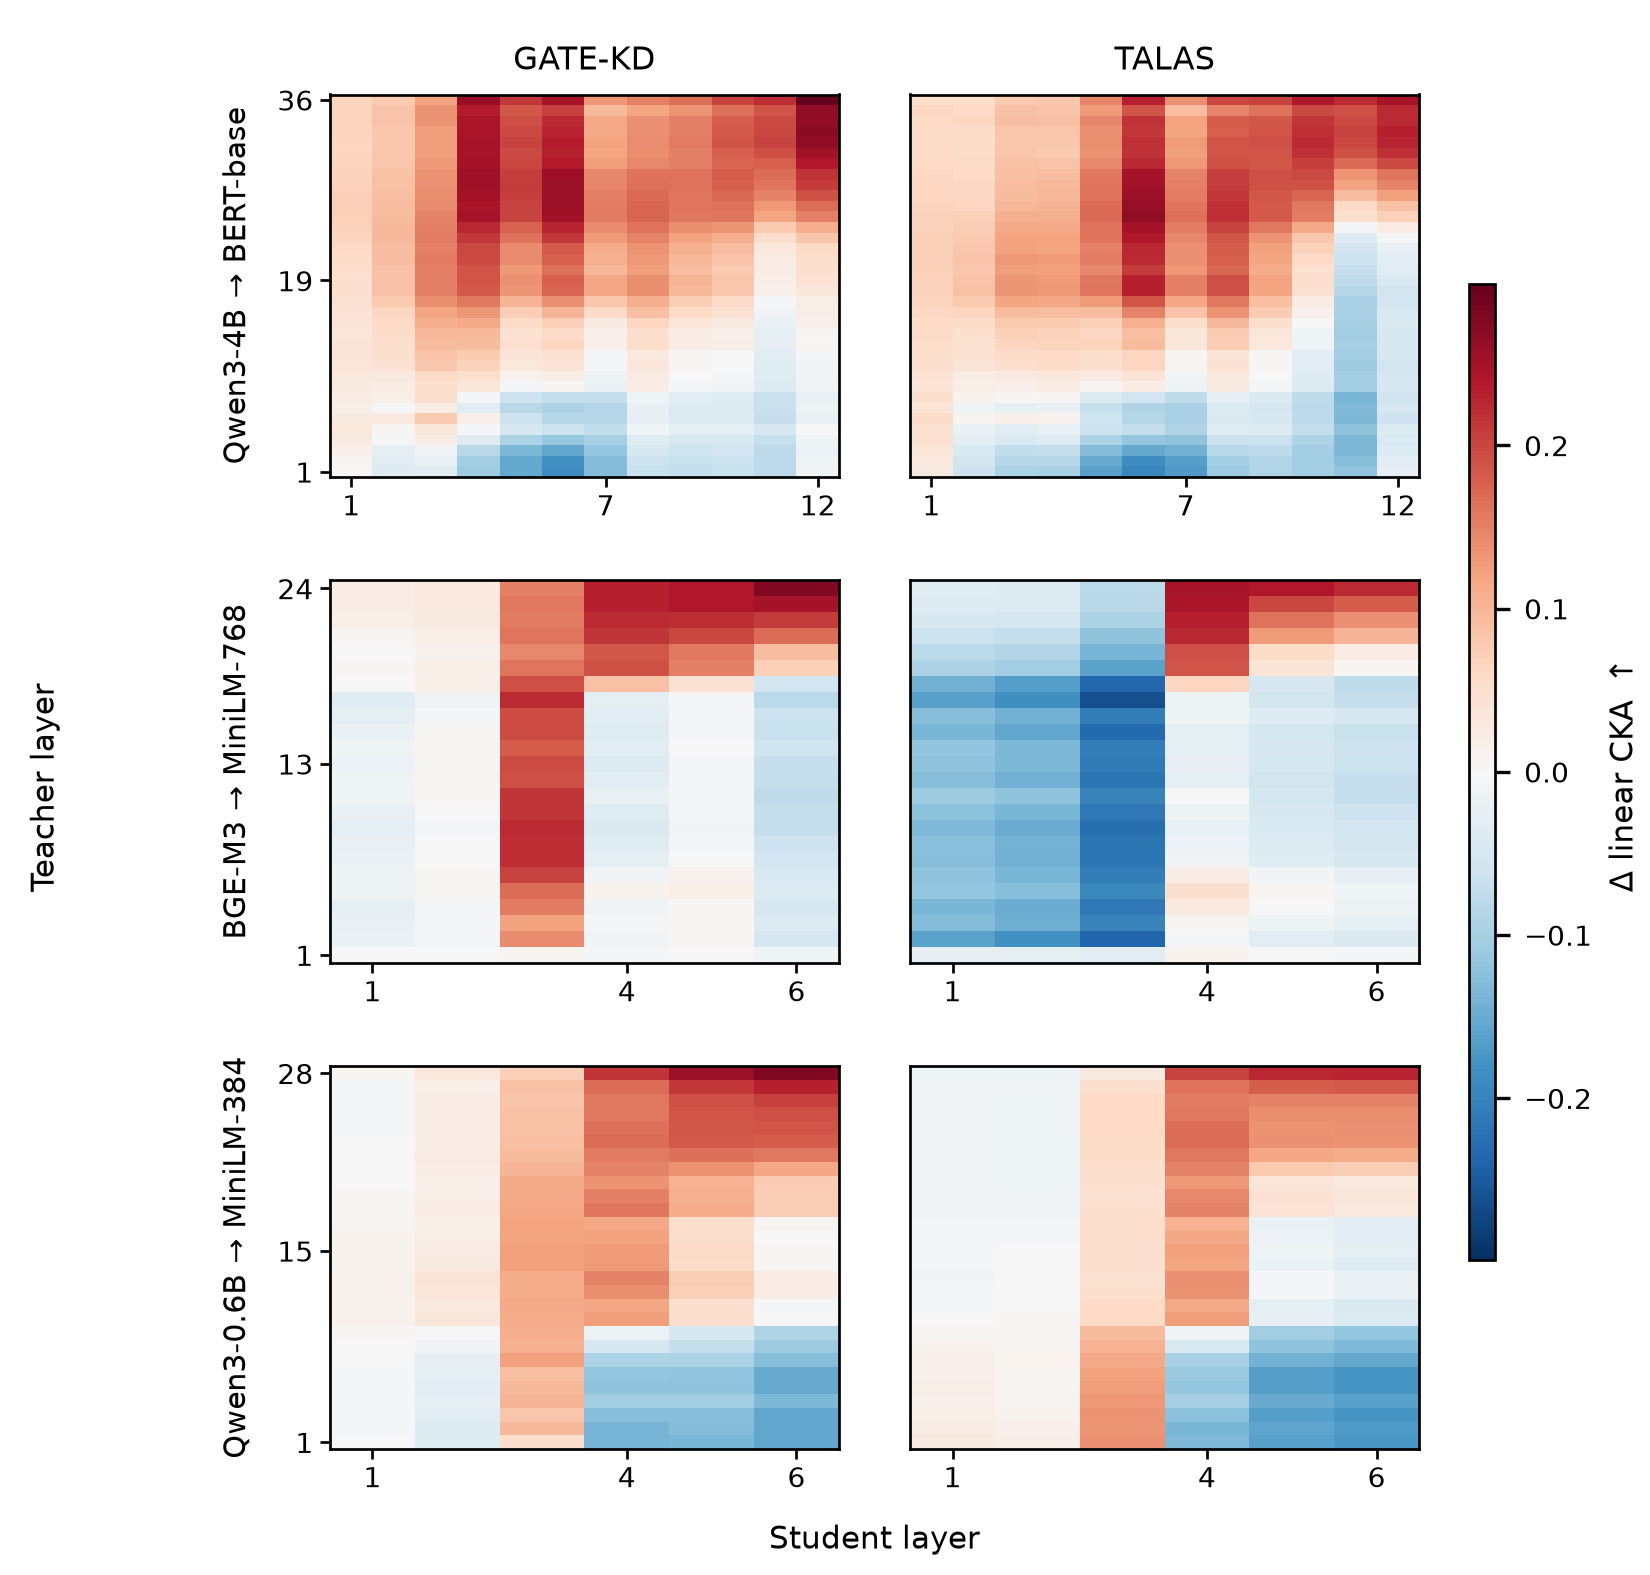
\includegraphics[width=0.82\textwidth]{figures/layerwise_delta_cka_all_pairs}
    \caption{Change in layerwise linear CKA relative to the pretrained
    student. Red and blue denote increased and decreased similarity,
    respectively.}
    \label{fig:layerwise-delta-cka}
\end{figure}

The changes are distributed across multiple later student layers rather than
being confined to a single teacher--student layer pair. This pattern is
consistent with endpoint supervision inducing an internal reorganization of
the student despite the absence of explicit intermediate-layer matching. Some
layer pairs decrease in CKA, so the result does not imply uniformly stronger
alignment at every depth. Moreover, CKA is descriptive and does not establish
that the observed internal changes cause the downstream improvements.

\FloatBarrier
\section{PCA Centering, Whitening, and Random-Subspace Controls}
\label{app:pca-controls}

We isolate preprocessing of the fixed endpoint interface in configuration (c).
Every row uses the endpoint-only objective, the same student, corpus, optimizer,
training schedule, and epoch-wise Procrustes updates. These are endpoint-only
controls, so the reference row is not labeled as GATE-KD or Ours; those names
refer to the full endpoint-plus-$H_0$ method in the main tables. The reference
estimates its principal directions from the centered cache but applies the
resulting linear map without subtracting the cache mean. ``Mean-subtracted
PCA'' applies that
mean subtraction as in the textbook affine PCA transform, while ``PCA
whitening'' additionally rescales each retained coordinate by the inverse square
root of its fitted eigenvalue. The random controls replace the PCA subspace with
three independent Haar-random subspaces of the same rank. Results are averaged
over the same three training seeds within each row; random-map draws remain
separate rather than being treated as additional training seeds.

% Sources: PCA + Procrustes reference from Table 3; remaining rows from
% review_h0_pca_controls_20260906-104859, PCA-family rows only.
\begin{table}[!htbp]
  \centering
  \caption{PCA preprocessing and subspace controls with endpoint-only
  supervision and Procrustes alignment in configuration (c). Scores are mean
  $\pm$ sample standard deviation over three seeds; random-subspace draws are
  shown separately. Best values are bold.}
  \label{tab:pca-preprocessing}
  \small
  \newcommand{\pcell}[2]{#1{\tiny $\pm$ #2}}
  \setlength{\tabcolsep}{4.5pt}
  \begin{tabular}{@{}lcccc@{}}
    \toprule
    Interface & Retained energy $\uparrow$ & Avg. IOD $\uparrow$
    & Avg. OOD $\uparrow$ & Avg. $\uparrow$ \\
    \midrule
    PCA $+$ Procrustes (reference)
      & 0.928 & \pcell{67.76}{0.05} & \pcell{77.54}{0.07}
      & \pcell{\textbf{74.28}}{0.03} \\
    Mean-subtracted PCA
      & 0.928 & \pcell{66.85}{0.15} & \pcell{74.95}{0.02} & \pcell{72.25}{0.06} \\
    PCA whitening
      & 0.928 & \pcell{\textbf{68.14}}{0.33} & \pcell{75.83}{0.08}
      & \pcell{73.26}{0.16} \\
    Random subspace (draw 0)
      & 0.381 & \pcell{67.38}{0.07} & \pcell{77.28}{0.06} & \pcell{73.98}{0.06} \\
    Random subspace (draw 1)
      & 0.376 & \pcell{67.41}{0.17} & \pcell{77.47}{0.05} & \pcell{74.12}{0.04} \\
    Random subspace (draw 2)
      & 0.374 & \pcell{67.48}{0.07} & \pcell{76.95}{0.08} & \pcell{73.79}{0.03} \\
    Uncentered SVD
      & \textbf{0.945} & \pcell{67.59}{0.22}
      & \pcell{\textbf{77.61}}{0.01} & \pcell{74.27}{0.08} \\
    \bottomrule
  \end{tabular}
\end{table}


Mean subtraction causes the largest degradation, particularly on the six OOD
benchmarks. Whitening recovers part of that loss and improves Avg.~IOD over the
reference, but remains lower on Avg.~OOD and overall Avg. The PCA reference
exceeds all three random draws despite retaining the same rank. Uncentered SVD
attains a numerically indistinguishable overall score, differing from the
Table~\ref{tab:interface-families} reference by 0.01 points. We
therefore retain the evaluated interface, while interpreting this control as
evidence for preserving the mean component at application time rather than as
evidence that fit-time centering is uniquely optimal.

\section{Target-Rank Sensitivity at Fixed Student Width}
\label{app:target-rank}

We isolate the subspace selected by the endpoint interface in configuration
(c). The student architecture, 384-dimensional output, distillation corpus,
optimizer, training schedule, and Procrustes updates remain fixed, while the
retained PCA rank varies over $k\in\{64,128,256,384\}$. This experiment uses
the endpoint-only objective. Targets with $k<384$ are embedded in the native
student space by appending zero coordinates before Procrustes alignment. This
padding preserves their Gram matrix and active rank, and does not change the
capacity or width of the student.

Retained energy is measured on the complete teacher cache. On a fixed sample
of 2{,}048 normalized teacher embeddings $T$, we measure the normalized
squared Gram distortion
$\lVert TT^\top-Y_kY_k^\top\rVert_F^2/\lVert TT^\top\rVert_F^2$, where $Y_k$
is the normalized rank-$k$ PCA target. We also report the normalized rank
floor $\sum_{j>k}\sigma_j(T)^4/\sum_j\sigma_j(T)^4$ from
Equation~\ref{eq:gram-lower-bound}. The Gram quantities are independent of
the orthogonal gauge and are therefore computed once, while downstream scores
are averaged over three seeds.

Figure~\ref{fig:target-rank} shows monotonic changes in all three quantities.
Increasing $k$ from 64 to 384 raises retained teacher energy from 59.32\% to
92.84\%, reduces normalized Gram distortion from 6.797\% to 0.086\%, and
improves Avg. from 72.57 to 74.27. The intermediate ranks 128 and 256 attain
73.77 and 74.21 Avg., respectively. Most of the downstream benefit is therefore
recovered by rank 256, with the final increase to rank 384 contributing only
0.06 points in this configuration.

\begin{figure}[H]
    \centering
    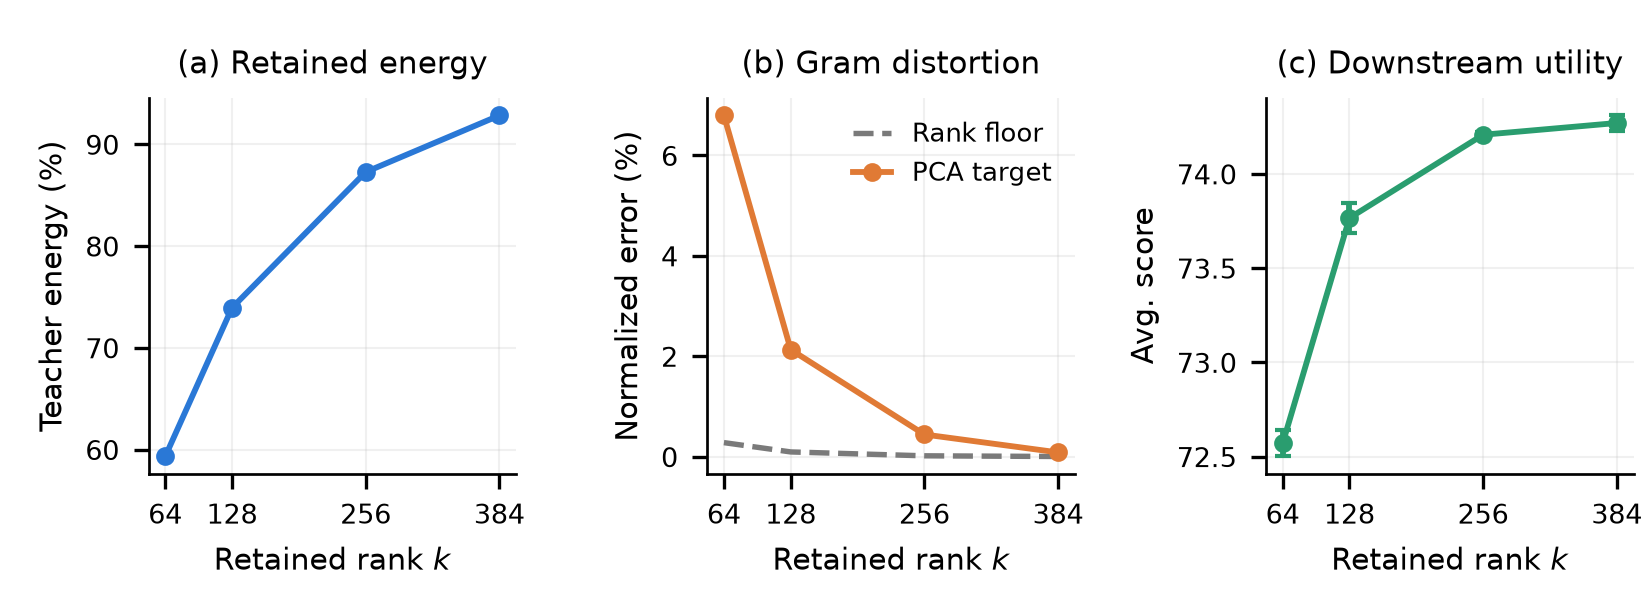
\includegraphics[width=0.85\textwidth]{figures/width_bottleneck}
    \caption{Sensitivity to retained PCA rank at fixed student width in
    configuration (c). Downstream scores show mean $\pm$ sample standard
    deviation over three seeds.}
    \label{fig:target-rank}
\end{figure}

PCA distortion remains roughly 21--25 times above the rank floor because its
objective differs from normalized Gram approximation; the floor bounds
irreducible error rather than predicting this interface's distortion.
Increasing rank improves geometry and utility with diminishing returns. With
the student architecture fixed, this is target-rank sensitivity, not a width
ablation.

% Supporting and extended tables, in presentation order.
% Sources: runs/sensitivity_s1_lambda_h0.csv, runs/sensitivity_s2_fit_set.csv,
% and runs/ablations_by_cell.csv for source/non-source aggregates.
% Current-code ablation suite: paper_ablations_15k_h200_gpu0-5_20260909-061547.
\begin{table}[t]
    \caption{Sensitivity analyses for configuration (c). Panel (a) varies the
    structural weight; panel (b) varies the representative fit-set size.
    Results are mean $\pm$ sample standard deviation over three seeds; best
    values in each panel are bold.}
    \label{tab:sensitivity-controls}
    \tablebody
    \begin{tabular}{@{}lccc@{}}
        \toprule
        Setting & Source $\uparrow$ & Non-source $\uparrow$ & Overall $\uparrow$ \\
        \midrule
        \multicolumn{4}{@{}l}{\textit{(a) Structural weight $\lambda_{H_0}$}} \\
        \midrule
        0
        & \meanstd{67.61}{0.09} & \meanstd{77.57}{0.06} & \meanstd{74.25}{0.01} \\
        0.1
        & \meanstd{68.13}{0.17} & \meanstd{77.75}{0.04} & \meanstd{74.54}{0.03} \\
        0.3
        & \meanstd{68.72}{0.28} & \meanstd{77.85}{0.06} & \meanstd{74.81}{0.05} \\
        0.5
        & \meanstd{\tablebest{68.80}}{0.16}
        & \meanstd{\tablebest{77.89}}{0.01}
        & \meanstd{\tablebest{74.86}}{0.06} \\
        1.0
        & \meanstd{68.38}{0.17} & \meanstd{77.75}{0.00} & \meanstd{74.63}{0.06} \\
        \midrule
        \multicolumn{4}{@{}l}{\textit{(b) Representative fit-set size}} \\
        \midrule
        2{,}048
        & \meanstd{68.69}{0.15} & \meanstd{77.62}{0.10} & \meanstd{74.65}{0.05} \\
        4{,}096
        & \meanstd{68.79}{0.07} & \meanstd{77.77}{0.05} & \meanstd{74.78}{0.05} \\
        8{,}192
        & \meanstd{68.55}{0.09} & \meanstd{77.84}{0.04} & \meanstd{74.75}{0.01} \\
        14{,}760
        & \meanstd{\tablebest{68.80}}{0.16}
        & \meanstd{\tablebest{77.89}}{0.01}
        & \meanstd{\tablebest{74.86}}{0.06} \\
        \bottomrule
    \end{tabular}
\end{table}

\begin{table}[t]
    \caption{Nine-task results with the 100K distillation corpus. Distilled
    students report mean $\pm$ standard deviation over three seeds; best and
    second-best results are bold and underlined.}
    \label{tab:main-results-100k}
    \widetablebody
    \begin{tabular}{@{}lcccccccccc@{}}
        \toprule
        & \multicolumn{3}{c}{Classification (F1)}
        & \multicolumn{3}{c}{Pair Classification (AP)}
        & \multicolumn{3}{c}{STS (Spearman)}
        & \\
        \cmidrule(lr){2-4}\cmidrule(lr){5-7}\cmidrule(lr){8-10}
        Method
        & Banking77
        & Tweet
        & Emotion
        & MRPC
        & SciTail
        & WiC
        & SICK
        & STS12
        & STS-B
        & Avg. \\
        \midrule
        \multicolumn{11}{@{}c}{\textit{(a) Qwen3-Embedding-4B $\rightarrow$ BERT-base (109M)}} \\
        \midrule
        Teacher
        & 93.26
        & 71.04
        & 69.08
        & 84.80
        & 91.77
        & 66.79
        & 83.43
        & 82.55
        & 86.87
        & 81.07 \\
        Student (pre-KD)
        & 84.33
        & 67.08
        & 47.79
        & 77.36
        & 67.74
        & 59.22
        & 42.43
        & 21.54
        & 20.29
        & 54.20 \\
        \midrule
        RKD
        & \meanstdstacked{92.23}{0.15}
        & \meanstdstacked{71.96}{0.18}
        & \meanstdstacked{63.79}{0.40}
        & \meanstdstacked{85.00}{0.04}
        & \meanstdstacked{80.27}{0.38}
        & \meanstdstacked{66.31}{0.10}
        & \meanstdstacked{79.32}{0.02}
        & \meanstdstacked{71.72}{0.16}
        & \meanstdstacked{77.70}{0.20}
        & \meanstdstacked{76.48}{0.04} \\
        Stella
        & \meanstdstacked{90.02}{0.15}
        & \meanstdstacked{71.90}{0.22}
        & \meanstdstacked{60.14}{0.45}
        & \meanstdstacked{\tablesecond{85.96}}{0.05}
        & \meanstdstacked{78.82}{0.27}
        & \meanstdstacked{\tablesecond{69.93}}{0.13}
        & \meanstdstacked{76.53}{0.23}
        & \meanstdstacked{69.79}{0.12}
        & \meanstdstacked{77.22}{0.16}
        & \meanstdstacked{75.59}{0.10} \\
        CDM
        & \meanstdstacked{89.16}{0.04}
        & \meanstdstacked{69.63}{0.23}
        & \meanstdstacked{53.74}{0.13}
        & \meanstdstacked{85.57}{0.08}
        & \meanstdstacked{71.22}{0.19}
        & \meanstdstacked{\tablebest{70.04}}{0.05}
        & \meanstdstacked{71.26}{0.29}
        & \meanstdstacked{66.97}{0.21}
        & \meanstdstacked{73.69}{0.38}
        & \meanstdstacked{72.36}{0.13} \\
        DSKD
        & \meanstdstacked{88.87}{0.07}
        & \meanstdstacked{69.05}{0.09}
        & \meanstdstacked{54.02}{0.56}
        & \meanstdstacked{85.90}{0.05}
        & \meanstdstacked{70.02}{0.31}
        & \meanstdstacked{69.63}{0.21}
        & \meanstdstacked{71.07}{0.10}
        & \meanstdstacked{66.52}{0.17}
        & \meanstdstacked{73.52}{0.01}
        & \meanstdstacked{72.07}{0.03} \\
        EMO
        & \meanstdstacked{84.96}{0.84}
        & \meanstdstacked{68.93}{0.65}
        & \meanstdstacked{54.80}{1.52}
        & \meanstdstacked{85.05}{0.04}
        & \meanstdstacked{65.75}{0.22}
        & \meanstdstacked{68.80}{0.13}
        & \meanstdstacked{62.00}{2.71}
        & \meanstdstacked{61.75}{1.85}
        & \meanstdstacked{69.54}{0.37}
        & \meanstdstacked{69.07}{0.89} \\
        TALAS
        & \meanstdstacked{\tablesecond{93.12}}{0.13}
        & \meanstdstacked{\tablebest{74.67}}{0.38}
        & \meanstdstacked{\tablesecond{71.42}}{0.26}
        & \meanstdstacked{\tablebest{86.30}}{0.01}
        & \meanstdstacked{\tablesecond{87.06}}{0.12}
        & \meanstdstacked{68.09}{0.02}
        & \meanstdstacked{\tablesecond{80.29}}{0.03}
        & \meanstdstacked{\tablesecond{76.34}}{0.01}
        & \meanstdstacked{\tablesecond{82.26}}{0.05}
        & \meanstdstacked{\tablesecond{79.95}}{0.08} \\
        \midrule
        \tablebest{GATE-KD}
        & \meanstdstacked{\tablebest{93.47}}{0.12}
        & \meanstdstacked{\tablesecond{74.18}}{0.25}
        & \meanstdstacked{\tablebest{72.50}}{0.47}
        & \meanstdstacked{85.45}{0.08}
        & \meanstdstacked{\tablebest{87.24}}{0.12}
        & \meanstdstacked{66.57}{0.08}
        & \meanstdstacked{\tablebest{81.85}}{0.06}
        & \meanstdstacked{\tablebest{76.40}}{0.07}
        & \meanstdstacked{\tablebest{82.52}}{0.08}
        & \meanstdstacked{\tablebest{80.02}}{0.03} \\
        \midrule
        \multicolumn{11}{@{}c}{\textit{(b) BGE-M3 $\rightarrow$ MiniLMv2-H768 (66M)}} \\
        \midrule
        Teacher
        & 93.49
        & 73.75
        & 69.03
        & 85.80
        & 91.87
        & 61.46
        & 79.18
        & 78.74
        & 84.86
        & 79.80 \\
        Student (pre-KD)
        & 81.18
        & 71.30
        & 48.85
        & 79.66
        & 65.06
        & 60.89
        & 49.46
        & 26.76
        & 24.12
        & 56.36 \\
        \midrule
        RKD
        & \meanstdstacked{91.68}{0.06}
        & \meanstdstacked{74.57}{0.40}
        & \meanstdstacked{62.45}{0.75}
        & \meanstdstacked{85.81}{0.08}
        & \meanstdstacked{79.81}{0.17}
        & \meanstdstacked{63.57}{0.13}
        & \meanstdstacked{76.91}{0.05}
        & \meanstdstacked{69.54}{0.11}
        & \meanstdstacked{75.56}{0.09}
        & \meanstdstacked{75.54}{0.10} \\
        Stella
        & \meanstdstacked{88.72}{0.41}
        & \meanstdstacked{73.43}{0.23}
        & \meanstdstacked{61.63}{0.29}
        & \meanstdstacked{86.39}{0.08}
        & \meanstdstacked{74.13}{0.31}
        & \meanstdstacked{\tablesecond{66.98}}{0.27}
        & \meanstdstacked{73.32}{0.07}
        & \meanstdstacked{68.30}{0.12}
        & \meanstdstacked{72.66}{0.14}
        & \meanstdstacked{73.95}{0.04} \\
        CDM
        & \meanstdstacked{87.64}{0.23}
        & \meanstdstacked{70.82}{0.14}
        & \meanstdstacked{56.37}{0.57}
        & \meanstdstacked{85.67}{0.08}
        & \meanstdstacked{67.69}{0.23}
        & \meanstdstacked{66.89}{0.20}
        & \meanstdstacked{70.15}{0.48}
        & \meanstdstacked{66.68}{0.26}
        & \meanstdstacked{69.49}{0.15}
        & \meanstdstacked{71.27}{0.10} \\
        DSKD
        & \meanstdstacked{86.69}{0.38}
        & \meanstdstacked{69.76}{0.22}
        & \meanstdstacked{56.98}{0.39}
        & \meanstdstacked{84.92}{0.07}
        & \meanstdstacked{66.75}{0.17}
        & \meanstdstacked{\tablebest{67.23}}{0.10}
        & \meanstdstacked{68.26}{0.45}
        & \meanstdstacked{66.28}{0.02}
        & \meanstdstacked{68.31}{0.35}
        & \meanstdstacked{70.58}{0.10} \\
        EMO
        & \meanstdstacked{87.17}{0.59}
        & \meanstdstacked{71.07}{0.22}
        & \meanstdstacked{59.32}{0.02}
        & \meanstdstacked{84.25}{0.41}
        & \meanstdstacked{67.89}{0.92}
        & \meanstdstacked{66.09}{0.18}
        & \meanstdstacked{69.04}{0.38}
        & \meanstdstacked{62.26}{1.77}
        & \meanstdstacked{66.47}{0.40}
        & \meanstdstacked{70.40}{0.35} \\
        TALAS
        & \meanstdstacked{\tablesecond{92.44}}{0.10}
        & \meanstdstacked{\tablesecond{75.58}}{0.15}
        & \meanstdstacked{\tablesecond{65.13}}{0.21}
        & \meanstdstacked{\tablebest{87.09}}{0.09}
        & \meanstdstacked{\tablesecond{85.39}}{0.14}
        & \meanstdstacked{64.39}{0.12}
        & \meanstdstacked{\tablesecond{78.14}}{0.06}
        & \meanstdstacked{\tablesecond{72.56}}{0.13}
        & \meanstdstacked{\tablebest{81.03}}{0.05}
        & \meanstdstacked{\tablesecond{77.97}}{0.03} \\
        \midrule
        \tablebest{GATE-KD}
        & \meanstdstacked{\tablebest{92.56}}{0.04}
        & \meanstdstacked{\tablebest{76.30}}{0.31}
        & \meanstdstacked{\tablebest{65.62}}{0.29}
        & \meanstdstacked{\tablesecond{86.58}}{0.05}
        & \meanstdstacked{\tablebest{87.20}}{0.06}
        & \meanstdstacked{63.43}{0.02}
        & \meanstdstacked{\tablebest{79.23}}{0.03}
        & \meanstdstacked{\tablebest{72.69}}{0.05}
        & \meanstdstacked{\tablesecond{80.60}}{0.13}
        & \meanstdstacked{\tablebest{78.24}}{0.05} \\
        \midrule
        \multicolumn{11}{@{}c}{\textit{(c) Qwen3-Embedding-0.6B $\rightarrow$ MiniLMv2-H384 (22M)}} \\
        \midrule
        Teacher
        & 92.51
        & 71.28
        & 65.80
        & 83.38
        & 90.09
        & 66.84
        & 80.65
        & 77.11
        & 84.59
        & 79.14 \\
        Student (pre-KD)
        & 67.03
        & 69.45
        & 42.90
        & 78.39
        & 64.55
        & 59.58
        & 47.60
        & 21.96
        & 22.08
        & 52.62 \\
        \midrule
        RKD
        & \meanstdstacked{89.74}{0.04}
        & \meanstdstacked{72.34}{0.22}
        & \meanstdstacked{57.99}{0.52}
        & \meanstdstacked{84.13}{0.12}
        & \meanstdstacked{75.20}{0.14}
        & \meanstdstacked{\tablebest{67.49}}{0.06}
        & \meanstdstacked{74.48}{0.03}
        & \meanstdstacked{68.12}{0.15}
        & \meanstdstacked{72.55}{0.14}
        & \meanstdstacked{73.56}{0.09} \\
        Stella
        & \meanstdstacked{85.74}{0.22}
        & \meanstdstacked{70.25}{0.07}
        & \meanstdstacked{53.48}{0.28}
        & \meanstdstacked{84.43}{0.04}
        & \meanstdstacked{71.23}{0.05}
        & \meanstdstacked{66.51}{0.14}
        & \meanstdstacked{70.96}{0.28}
        & \meanstdstacked{63.02}{0.04}
        & \meanstdstacked{67.42}{0.24}
        & \meanstdstacked{70.34}{0.02} \\
        CDM
        & \meanstdstacked{85.18}{0.08}
        & \meanstdstacked{69.14}{0.07}
        & \meanstdstacked{52.30}{0.26}
        & \meanstdstacked{84.02}{0.04}
        & \meanstdstacked{68.24}{0.23}
        & \meanstdstacked{66.57}{0.29}
        & \meanstdstacked{69.15}{0.13}
        & \meanstdstacked{63.05}{0.06}
        & \meanstdstacked{66.55}{0.10}
        & \meanstdstacked{69.36}{0.08} \\
        DSKD
        & \meanstdstacked{85.04}{0.14}
        & \meanstdstacked{69.21}{0.13}
        & \meanstdstacked{52.85}{0.36}
        & \meanstdstacked{84.34}{0.10}
        & \meanstdstacked{67.33}{0.24}
        & \meanstdstacked{65.98}{0.12}
        & \meanstdstacked{69.01}{0.13}
        & \meanstdstacked{63.46}{0.21}
        & \meanstdstacked{66.42}{0.09}
        & \meanstdstacked{69.29}{0.09} \\
        EMO
        & \meanstdstacked{85.08}{0.17}
        & \meanstdstacked{68.11}{0.10}
        & \meanstdstacked{53.96}{0.60}
        & \meanstdstacked{84.38}{0.16}
        & \meanstdstacked{65.48}{0.16}
        & \meanstdstacked{65.23}{0.17}
        & \meanstdstacked{68.61}{0.07}
        & \meanstdstacked{60.00}{0.82}
        & \meanstdstacked{65.38}{0.38}
        & \meanstdstacked{68.47}{0.15} \\
        TALAS
        & \meanstdstacked{\tablesecond{89.79}}{0.03}
        & \meanstdstacked{\tablesecond{73.87}}{0.17}
        & \meanstdstacked{\tablesecond{61.75}}{0.61}
        & \meanstdstacked{\tablebest{85.99}}{0.03}
        & \meanstdstacked{\tablesecond{82.07}}{0.09}
        & \meanstdstacked{65.79}{0.04}
        & \meanstdstacked{\tablesecond{75.67}}{0.05}
        & \meanstdstacked{\tablebest{73.91}}{0.03}
        & \meanstdstacked{\tablesecond{78.31}}{0.04}
        & \meanstdstacked{\tablesecond{76.35}}{0.08} \\
        \midrule
        \tablebest{GATE-KD}
        & \meanstdstacked{\tablebest{91.68}}{0.09}
        & \meanstdstacked{\tablebest{74.43}}{0.21}
        & \meanstdstacked{\tablebest{66.88}}{0.36}
        & \meanstdstacked{\tablesecond{85.00}}{0.06}
        & \meanstdstacked{\tablebest{83.46}}{0.02}
        & \meanstdstacked{\tablesecond{67.44}}{0.04}
        & \meanstdstacked{\tablebest{77.94}}{0.06}
        & \meanstdstacked{\tablesecond{72.17}}{0.02}
        & \meanstdstacked{\tablebest{78.36}}{0.07}
        & \meanstdstacked{\tablebest{77.48}}{0.04} \\
        \bottomrule
    \end{tabular}
\end{table}

\begin{table}[H]
    \caption{Training hyperparameters of the main experiments.}
    \label{tab:training-hyperparameters}
    \vspace{0.5em}
    \centering
    \scriptsize
    \setlength{\tabcolsep}{3pt}
    \begin{tabular}{@{}lccccc@{}}
        \toprule
        Method & Epochs & Batch & Learning rate & Optimizer & Warm-up \\
        \midrule
        RKD     & 5     & 128 & $7\times10^{-5}$ & AdamW & 0.06 \\
        Stella  & $2+3$ & 128 & $5\times10^{-5}$ & AdamW & 0.06 \\
        CDM     & 5     & 128 & $2\times10^{-5}$ & AdamW & 0.06 \\
        DSKD    & 5     & 128 & $2\times10^{-5}$ & AdamW & 0.06 \\
        EMO     & 5     & 128 & $1\times10^{-5}$ & AdamW & 0.10 \\
        TALAS   & 5     & 128 & $2\times10^{-5}$ & AdamW + adaptive SAM & 0.06 \\
        GATE-KD & 5     & 128 & $7\times10^{-5}$ & AdamW & 0.06 \\
        \bottomrule
    \end{tabular}
\end{table}



\end{document}
